%%%%%%%%%%%%%%%%%%%%%%%%%%%%%%%%%%%%%%%%
% datoteka diploma-vzorec.tex
%
% vzorčna datoteka za pisanje diplomskega dela v formatu LaTeX
% na UL Fakulteti za računalništvo in informatiko
%
% vkup spravil Gašper Fijavž, december 2010
% 
%
%
% verzija 12. februar 2014 (besedilo teme, seznam kratic, popravki Gašper Fijavž)
% verzija 10. marec 2014 (redakcijski popravki Zoran Bosnić)
% verzija 11. marec 2014 (redakcijski popravki Gašper Fijavž)
% verzija 15. april 2014 (pdf/a 1b compliance, not really - just claiming, Damjan Cvetan, Gašper Fijavž)
% verzija 23. april 2014 (privzeto cc licenca)
% verzija 16. september 2014 (odmiki strain od roba)
% verzija 28. oktober 2014 (odstranil vpisno številko)
% verija 5. februar 2015 (Literatura v kazalu, online literatura)
% verzija 25. september 2015 (angl. naslov v izjavi o avtorstvu)
% verzija 26. februar 2016 (UL izjava o avtorstvu)
% verzija 16. april 2016 (odstranjena izjava o avtorstvu)
% verzija 5. junij 2016 (Franc Solina dodal vrstice, ki jih je označil s svojim imenom)


\documentclass[a4paper, 12pt]{book}
%\documentclass[a4paper, 12pt, draft]{book}  Nalogo preverite tudi z opcijo draft, ki vam bo pokazala, katere vrstice so predolge!



\usepackage[utf8]{inputenc}   % omogoča uporabo slovenskih črk kodiranih v formatu UTF-8
\usepackage[slovene,english]{babel}    % naloži, med drugim, slovenske delilne vzorce

\usepackage{biblatex}
\addbibresource{literatura.bib}

\usepackage[pdftex]{graphicx}  % omogoča vlaganje slik različnih formatov
\graphicspath{ {./images/} }

\usepackage{float}          % poskrbi, na primer, za glave strani
\usepackage{csquotes}
\usepackage{fancyhdr}          % poskrbi, na primer, za glave strani
\usepackage{fancyvrb}          % poskrbi za underlined verbatim
\usepackage{amssymb}           % dodatni simboli
\usepackage{amsmath}           % eqref, npr.
\usepackage{hyperxmp}
%\usepackage[hyphens]{url}  % dodal Solina
%\usepackage{comment}       % dodal Solina
\usepackage[pdftex, colorlinks=true,
  						citecolor=black, filecolor=black, 
  						linkcolor=black, urlcolor=black,
  						pagebackref=false, 
  						pdfproducer={LaTeX}, pdfcreator={LaTeX}, hidelinks]{hyperref}
 
%\usepackage[separate-uncertainty=true,multi-part-units=repeat]{siunitx}

\usepackage{color}       % dodal Solina
\usepackage{soul}       % dodal Solina

%%%%%%%%%%%%%%%%%%%%%%%%%%%%%%%%%%%%%%%%
%	DIPLOMA INFO
%%%%%%%%%%%%%%%%%%%%%%%%%%%%%%%%%%%%%%%%
\newcommand{\ttitle}{Avtomatizacija delavniškega dnevnika}
\newcommand{\ttitleEn}{Workshop report automatisation}
\newcommand{\tsubject}{\ttitle}
\newcommand{\tsubjectEn}{\ttitleEn}
\newcommand{\tauthor}{Anej Lekše}
\newcommand{\tkeywords}{mobilni razvoj, glasovni asistenti, razpoznava glasu, informacijski sistemi}
\newcommand{\tkeywordsEn}{mobile development, voice assistants, voice recognition, information systems}


%%%%%%%%%%%%%%%%%%%%%%%%%%%%%%%%%%%%%%%%
%	HYPERREF SETUP
%%%%%%%%%%%%%%%%%%%%%%%%%%%%%%%%%%%%%%%%
\hypersetup{pdftitle={\ttitle}}
\hypersetup{pdfsubject=\ttitleEn}
\hypersetup{pdfauthor={\tauthor, al1617@student.uni-lj.si}}
\hypersetup{pdfkeywords=\tkeywordsEn}


 


%%%%%%%%%%%%%%%%%%%%%%%%%%%%%%%%%%%%%%%%
% postavitev strani
%%%%%%%%%%%%%%%%%%%%%%%%%%%%%%%%%%%%%%%%  

\addtolength{\marginparwidth}{-20pt} % robovi za tisk
\addtolength{\oddsidemargin}{40pt}
\addtolength{\evensidemargin}{-40pt}

\renewcommand{\baselinestretch}{1.3} % ustrezen razmik med vrsticami
\setlength{\headheight}{15pt}        % potreben prostor na vrhu
\renewcommand{\chaptermark}[1]%
{\markboth{\MakeUppercase{\thechapter.\ #1}}{}} \renewcommand{\sectionmark}[1]%
{\markright{\MakeUppercase{\thesection.\ #1}}} \renewcommand{\headrulewidth}{0.5pt} \renewcommand{\footrulewidth}{0pt}
\fancyhf{}
\fancyhead[LE,RO]{\sl \thepage} 
%\fancyhead[LO]{\sl \rightmark} \fancyhead[RE]{\sl \leftmark}
\fancyhead[RE]{\sc \tauthor}              % dodal Solina
\fancyhead[LO]{\sc Diplomska naloga}     % dodal Solina


\newcommand{\BibTeX}{{\sc Bib}\TeX}

%%%%%%%%%%%%%%%%%%%%%%%%%%%%%%%%%%%%%%%%
% naslovi
%%%%%%%%%%%%%%%%%%%%%%%%%%%%%%%%%%%%%%%%  


\newcommand{\autfont}{\Large}
\newcommand{\titfont}{\LARGE\bf}
\newcommand{\clearemptydoublepage}{\newpage{\pagestyle{empty}\cleardoublepage}}
\setcounter{tocdepth}{1}	      % globina kazala

%%%%%%%%%%%%%%%%%%%%%%%%%%%%%%%%%%%%%%%%
% konstrukti
%%%%%%%%%%%%%%%%%%%%%%%%%%%%%%%%%%%%%%%%  
\newtheorem{izrek}{Izrek}[chapter]
\newtheorem{trditev}{Trditev}[izrek]
\newenvironment{dokaz}{\emph{Dokaz.}\ }{\hspace{\fill}{$\Box$}}

%%%%%%%%%%%%%%%%%%%%%%%%%%%%%%%%%%%%%%%%%%%%%%%%%%%%%%%%%%%%%%%%%%%%%%%%%%%%%%%
%% PDF-A
%%%%%%%%%%%%%%%%%%%%%%%%%%%%%%%%%%%%%%%%%%%%%%%%%%%%%%%%%%%%%%%%%%%%%%%%%%%%%%%


%%%%%%%%%%%%%%%%%%%%%%%%%%%%%%%%%%%%%%%% 
% define medatata
%%%%%%%%%%%%%%%%%%%%%%%%%%%%%%%%%%%%%%%% 
\def\Title{\ttitle}
\def\Author{\tauthor, al1617@student.uni-lj.si}
\def\Subject{\ttitleEn}
\def\Keywords{\tkeywordsEn}

%%%%%%%%%%%%%%%%%%%%%%%%%%%%%%%%%%%%%%%% 
% \convertDate converts D:20080419103507+02'00' to 2008-04-19T10:35:07+02:00
%%%%%%%%%%%%%%%%%%%%%%%%%%%%%%%%%%%%%%%% 
\def\convertDate{%
    \getYear
}

{\catcode`\D=12
 \gdef\getYear D:#1#2#3#4{\edef\xYear{#1#2#3#4}\getMonth}
}
\def\getMonth#1#2{\edef\xMonth{#1#2}\getDay}
\def\getDay#1#2{\edef\xDay{#1#2}\getHour}
\def\getHour#1#2{\edef\xHour{#1#2}\getMin}
\def\getMin#1#2{\edef\xMin{#1#2}\getSec}
\def\getSec#1#2{\edef\xSec{#1#2}\getTZh}
\def\getTZh +#1#2{\edef\xTZh{#1#2}\getTZm}
\def\getTZm '#1#2'{%
    \edef\xTZm{#1#2}%
    \edef\convDate{\xYear-\xMonth-\xDay T\xHour:\xMin:\xSec+\xTZh:\xTZm}%
}

\expandafter\convertDate\pdfcreationdate 

%%%%%%%%%%%%%%%%%%%%%%%%%%%%%%%%%%%%%%%%
% get pdftex version string
%%%%%%%%%%%%%%%%%%%%%%%%%%%%%%%%%%%%%%%% 
\newcount\countA
\countA=\pdftexversion
\advance \countA by -100
\def\pdftexVersionStr{pdfTeX-1.\the\countA.\pdftexrevision}


%%%%%%%%%%%%%%%%%%%%%%%%%%%%%%%%%%%%%%%%
% XMP data
%%%%%%%%%%%%%%%%%%%%%%%%%%%%%%%%%%%%%%%%  
\usepackage{xmpincl}
\includexmp{pdfa-1b}

%%%%%%%%%%%%%%%%%%%%%%%%%%%%%%%%%%%%%%%%
% pdfInfo
%%%%%%%%%%%%%%%%%%%%%%%%%%%%%%%%%%%%%%%%  
\pdfinfo{%
    /Title    (\ttitle)
    /Author   (\tauthor, damjan@cvetan.si)
    /Subject  (\ttitleEn)
    /Keywords (\tkeywordsEn)
    /ModDate  (\pdfcreationdate)
    /Trapped  /False
}


%%%%%%%%%%%%%%%%%%%%%%%%%%%%%%%%%%%%%%%%%%%%%%%%%%%%%%%%%%%%%%%%%%%%%%%%%%%%%%%
%%%%%%%%%%%%%%%%%%%%%%%%%%%%%%%%%%%%%%%%%%%%%%%%%%%%%%%%%%%%%%%%%%%%%%%%%%%%%%%

\begin{document}
\selectlanguage{slovene}
\frontmatter
\setcounter{page}{1} %
\renewcommand{\thepage}{}       % preprecimo težave s številkami strani v kazalu
\newcommand{\sn}[1]{"`#1"'}                    % dodal Solina (slovenski narekovaji)

%%%%%%%%%%%%%%%%%%%%%%%%%%%%%%%%%%%%%%%%
%naslovnica
 \thispagestyle{empty}%
   \begin{center}
    {\large\sc Univerza v Ljubljani\\%
      Fakulteta za računalništvo in informatiko}%
    \vskip 10em%
    {\autfont \tauthor\par}%
    {\titfont \ttitle \par}%
    {\vskip 3em \textsc{DIPLOMSKO DELO\\[5mm]         % dodal Solina za ostale študijske programe
    VISOKOŠOLSKI STROKOVNI ŠTUDIJSKI PROGRAM\\ PRVE STOPNJE\\ RAČUNALNIŠTVO IN INFORMATIKA}\par}%
%    UNIVERZITETNI  ŠTUDIJSKI PROGRAM\\ PRVE STOPNJE\\ RAČUNALNIŠTVO IN INFORMATIKA}\par}%
%    INTERDISCIPLINARNI UNIVERZITETNI\\ ŠTUDIJSKI PROGRAM PRVE STOPNJE\\ RAČUNALNIŠTVO IN MATEMATIKA}\par}%
%    INTERDISCIPLINARNI UNIVERZITETNI\\ ŠTUDIJSKI PROGRAM PRVE STOPNJE\\ UPRAVNA INFORMATIKA}\par}%
%    INTERDISCIPLINARNI UNIVERZITETNI\\ ŠTUDIJSKI PROGRAM PRVE STOPNJE\\ MULTIMEDIJA}\par}%
    \vfill\null%
    {\large \textsc{Mentor}: doc.\ dr.  Andrej Brodnik\par}%
   %{\large \textsc{Somentor}:  izr.\ prof.\ dr. Martin Krpan \par}%
    {\vskip 2em \large Ljubljana, 2020 \par}%
\end{center}
% prazna stran
%\clearemptydoublepage      % dodal Solina (izjava o licencah itd. se izpiše na hrbtni strani naslovnice)

%%%%%%%%%%%%%%%%%%%%%%%%%%%%%%%%%%%%%%%%
%copyright stran
\thispagestyle{empty}
\vspace*{8cm}

\noindent
{\sc Copyright}. 
Rezultati diplomske naloge so intelektualna lastnina avtorja in Fakultete za računalništvo in informatiko Univerze v Ljubljani.
Za objavo in koriščenje rezultatov diplomske naloge je potrebno pisno privoljenje avtorja, Fakultete za računalništvo in informatiko ter mentorja.

\begin{center}
\mbox{}\vfill
\emph{Besedilo je oblikovano z urejevalnikom besedil \LaTeX.}
\end{center}
% prazna stran
\clearemptydoublepage

%%%%%%%%%%%%%%%%%%%%%%%%%%%%%%%%%%%%%%%%
% stran 3 med uvodnimi listi
\thispagestyle{empty}
\vspace*{4cm}

\noindent
Fakulteta za računalništvo in informatiko izdaja naslednjo nalogo:
\medskip
\begin{tabbing}
\hspace{32mm}\= \hspace{6cm} \= \kill




Tematika naloge:
\end{tabbing}
%Besedilo teme diplomskega dela študent prepiše iz študijskega informacijskega sistema, kamor ga je vnesel mentor. V nekaj stavkih bo opisal, kaj pričakuje od kandidatovega diplomskega dela. Kaj so cilji, kakšne metode uporabiti, morda bo zapisal tudi ključno literaturo.
Preveri ali so glasovni asistenti v trenutnem stanju primerni za pomoč pri pisanju delavniških dnevnikov.
Seznani se z obstoječimi programskimi rešitvami in jih analiziraj.
Po analizi področja se loti izdelave svojega sistema za pisanje delavniških dnevnikov, ki vključuje glasovnega asistenta.
\vspace{15mm}



\vspace{2cm}

% prazna stran
\clearemptydoublepage

% zahvala
\thispagestyle{empty}\mbox{}\vfill\null\it%
\noindent
Na tem mestu zapišite, komu se zahvaljujete za izdelavo diplomske naloge. Pazite, da ne boste koga pozabili. Utegnil vam bo zameriti. Temu se da izogniti tako, da celotno zahvalo izpustite.
\rm\normalfont

% prazna stran
\clearemptydoublepage

%%%%%%%%%%%%%%%%%%%%%%%%%%%%%%%%%%%%%%%%
% posvetilo, če sama zahvala ne zadošča :-)
\thispagestyle{empty}\mbox{}{\vskip0.20\textheight}\mbox{}\hfill\begin{minipage}{0.55\textwidth}%
%Svoji dragi Alenčici.
	Kavi. Hvala.
\normalfont\end{minipage}

% prazna stran
\clearemptydoublepage


%%%%%%%%%%%%%%%%%%%%%%%%%%%%%%%%%%%%%%%%
% kazalo
\pagestyle{empty}
\def\thepage{}% preprecimo tezave s stevilkami strani v kazalu
\tableofcontents{}


% prazna stran
\clearemptydoublepage

%%%%%%%%%%%%%%%%%%%%%%%%%%%%%%%%%%%%%%%%
% seznam kratic

\chapter*{Seznam uporabljenih kratic}  % spremenil Solina, da predolge vrstice ne gredo preko desnega roba

% \begin{comment}
% \begin{tabular}{l|l|l}
%   {\bf kratica} & {\bf angleško} & {\bf slovensko} \\ \hline
%   % after \\: \hline or \cline{col1-col2} \cline{col3-col4} ...
%   {\bf CA} & classification accuracy & klasifikacijska točnost \\
%   {\bf DBMS} & database management system & sistem za upravljanje podatkovnih baz \\
%   {\bf SVM} & support vector machine & metoda podpornih vektorjev \\
%   \dots & \dots & \dots \\
% \end{tabular}
% \end{comment}

\noindent\begin{tabular}{p{0.1\textwidth}|p{.4\textwidth}|p{.4\textwidth}}    % po potrebi razširi prvo kolono tabele na račun drugih dveh!
  {\bf kratica} & {\bf angleško}                             & {\bf slovensko} \\ \hline
  {\bf API} & Application Programming Interface & vmesnik za programiranje aplikacije \\
  {\bf AWS} & Amazon Web Services & Amazonove spletne storitve \\
  {\bf FIFO} & First In First Out & Prvi not, prvi ven \\
  {\bf HTML} & HyperText Markup Language & Označitveni jezik za hipertekst \\
  {\bf HTTP} & HyperText Transfer Protocol & Protokol za prenos hiperteksta \\
  {\bf HTTPS} & HyperText Transfer Protocol Secure & Protokol za prenos hiperteksta, varna različica? \\
  {\bf IP} & Internet Protocol & Internetni protokol \\
  {\bf JSON} & JavaScript Object Notation & JavaScript zapis objektov\\
  {\bf JWT} & JSON Web Token & JSON spletni žeton \\
  {\bf LIMS} & Laboratory Information Management System & laboratorijski sistem za uporavljanje informacij \\
  {\bf MIT} & Massachusetts Institute of Technology & Tehnološki inštitut Massachusettsa \\
  {\bf MVVM} & Model View View-Model & Model Pogled Pogled-Model \\
  {\bf NLU} & Natural Langugage Understanding & Razumevanje naravnega govora \\
  {\bf SQS} & Simple Queue Service & preprosta vrstna storitev \\
  {\bf UI} & User Interface & uporabniški vmesnik \\
  {\bf URL} & Universal Resource Locator & Univerzalni lokator virov \\
  {\bf VUI} & Voice User Interface & glasovni uporabniški vmesnik \\
  {\bf XAML} & Extensible Application Markup Langugage & razširljiv aplikacijski označitveni? jezik \\
%  \dots & \dots & \dots \\
\end{tabular}


% prazna stran
\clearemptydoublepage

%%%%%%%%%%%%%%%%%%%%%%%%%%%%%%%%%%%%%%%%
% povzetek
\addcontentsline{toc}{chapter}{Povzetek}
\chapter*{Povzetek}

\noindent\textbf{Naslov:} \ttitle
\bigskip

\noindent\textbf{Avtor:} \tauthor
\bigskip

%Dober povzetek vključuje: (1) kratek opis obravnavanega problema, (2) kratek opis vašega pristopa za reševanje tega problema in (3) (najbolj uspešen) rezultat ali prispevek magistrske naloge.

\noindent Diplomsko delo obravnava področje vpeljave komercialno dostopnih glasovnih asistentov v proces pisanja delavniškega dnevnika.
V nalogi raziščemo, ali vpeljava glasovnega asistenta v računalniški sistem pospeši delo s tem sistemom. 
Cilj je implementirati in preizkusiti računalniški sistem z glasovnim asistentom, s pomočjo katerega lahko narekujemo zapiske med delom. 
Te zapiske pa lahko naknandno urejamo s pomočjo mobilne aplikacije.
Uporabili bomo Amazon Alexo zaradi enostavne izdelave lastnih programov (t.i. ''Skill-ov'').
% Ugotovili smo, da je specializiran sistem za pisanje opisov tehnološkega postopka lahko dobra alternativa pisanju teh dokumentov s pisarniškimi programi ali na list papirja.
Ugotovili smo, da Amazon Alexa ni bila zmožna razpoznati izgovorjenih stavkov z veliko variirajočimi besedami.
Uspešna je bila pri razpoznavanju stavkov, ki so se v večini ali v celoti ujemali z naučenim razpoznavnim modelom.
Kljub temu, je čas, ki je potreben, da Alexa razpozna prejet glasovni ukaz prepočasen, da bi bil sistem učinkovit.
\bigskip

\noindent\textbf{Ključne besede:} \tkeywords.
% prazna stran
\clearemptydoublepage

%%%%%%%%%%%%%%%%%%%%%%%%%%%%%%%%%%%%%%%%
% abstract
\selectlanguage{english}
\addcontentsline{toc}{chapter}{Abstract}
\chapter*{Abstract}

\noindent\textbf{Title:} \ttitleEn
\bigskip

\noindent\textbf{Author:} \tauthor
\bigskip

// TODO fix 

\noindent This thesis deals with the process of optimising the process of writing a workshop report.
The goal of thesis was testing a system with a voice assistant that could be used to take notes during work.
These notes can be edited and ordered via a mobile application.
We have used Amazon Alexa as it offers simple programming with Alexa Skills.
We discovered that a specialised system for writing workshop reports can be an improvement over writing them with office suites or using pen and paper.
We discovered that Amazon Alexa was unsuitable for a literal dictation of longer, largely varying text.
It was successful at recognising phrases that fully or mostly matched its learned model.
Regardless, Alexa's ability to process custom voice commands, at the time of this research, was too slow to be deemed efficient.

\bigskip

\noindent\textbf{Keywords:} \tkeywordsEn.
\selectlanguage{slovene}
% prazna stran
\clearemptydoublepage

%%%%%%%%%%%%%%%%%%%%%%%%%%%%%%%%%%%%%%%%
\mainmatter
\setcounter{page}{1}
\pagestyle{fancy}

\chapter{Uvod}
\section{Opis domene raziskave}

Diplomsko delo obravnava področje vpeljave glasovnih asistentov v programske rešitve kot sredstvo za izboljšanje učinkovitosti dela.

Za področje, ki ga želimo izboljšati smo si izbrali pisanje delavniškega dnevnika ali opisa tehnološkega postopka.
Kljub temu se bo naš sistem z minimalnimi modifikacijami lahko uporabil tudi za pisanje drugačnih vrst poročil in navodil.
Med te spadajo kuharski recepti, laboratorijski dnevniki, itd.

Opis tehnološkega postopka ali delavniški dnevnik je dokument, ki po korakih nedvoumno predstavi postopek izdelave izdelka.
Delavniški dnevniki imajo lahko definirane tudi kontrolne postopke za izdelek, orodje, ki ga rabimo za izdelavo in seznam možnih nevarnosti pri delu.

Delavniški dnevnik je sestavljen iz zaporedja korakov, ki si sledijo v časovnem zaporedju.
Vsak korak sestavljata opis postopka in predvideno trajanje.
Koraki lahko vsebujejo tudi slikovne razlage.

Opisi tehnološkega postopka se najpogosteje uporabljajo v proizvodnih obratih tovarn.

V sklopu diplomske naloge smo želeli izdelati in raziskati učinkovitost specializiranega sistema za pisanje delavniških dnevnikov.
Ta sistem, bi sestavljali glasovni asistent, ki bi služil za narekovanje opomb, mobilna aplikacija, preko katere bi lahko urejali zapiske in strežnik, ki bi hranil podatke.

Raziskati želimo predpostavko, da lahko z učinkovito uporabo glasovnega asistenta zmanjšamo čas interakcije z mobilno aplikacijo.


\section{Struktura diplomske naloge}

Diplomsko delo pričenjamo s predstavitvijo področja raziskave in kratko opišemo problem in možno rešitev. 
Postavimo si hipotezo.
% V sklopu te diplomski naloge bomo raziskali, ali je specializirana programska rešitev z glasovnim asistentom in mobilno aplikacijo primerno orodje za učinkovito pisanje delavniških dnevnikov.

Začnemo z raziskavo že obstoječih rešitev za pisanje opisa tehnološkega postopka.
Nato opišemo, kaj trenutne rešitve te problematike ponujajo in njihove prednosti in slabosti.

V naslednjem poglavju se lotimo načrtovanja specializiranega sistema z glasovnim asistentom za pomoč pri pisanju poročil.
Nato se lotimo opisa tehnologij, ki smo jih pri pisanju diplome uporabili.
Natančno definiramo funkcionalnosti sistema, utemeljimo odločitev za izbiro Amazon Alexe, AWS SQS, AWS Lambda in ogrodja Xamarin.

Nato izdelamo Alexa ''Skill'', strežniški program in mobilno aplikacijo.
Funkcionalnosti sistema testiramo in analiziramo.

V predzadnjem poglavju opišemo možnosti nadaljnjega razvoja projekta.

\chapter{Pregled problema in rešitve}

\section{Problem}

\subsection {Kaj je delavniški dnevnik?}

Opis tehnološkega postopka ali delavniški dnevnik je dokument, ki po korakih nedvoumno predstavi postopek izdelave izdelka.
Delavniški dnevniki imajo lahko definirane tudi kontrolne postopke za izdelek, orodje, ki ga rabimo za izdelavo in seznam možnih nevarnosti pri delu.

Delavniški dnevnik je sestavljen iz zaporedja korakov, ki si sledijo v časovnem zaporedju.
Vsak korak je sestavljata opis postopka in predvideno trajanje.
Koraki lahko vsebujejo tudi slikovne razlage.

Opisi tehnološkega postopka se najpogosteje uporabljajo v proizvodnih obratih tovarn.

\subsection{Primer}
Spodnja slika (Slika \ref{sap_2}) prikazuje primer opisa tehnološkega postopka za izdelavo hladilnika.

\begin{figure}[H]
\begin{center}
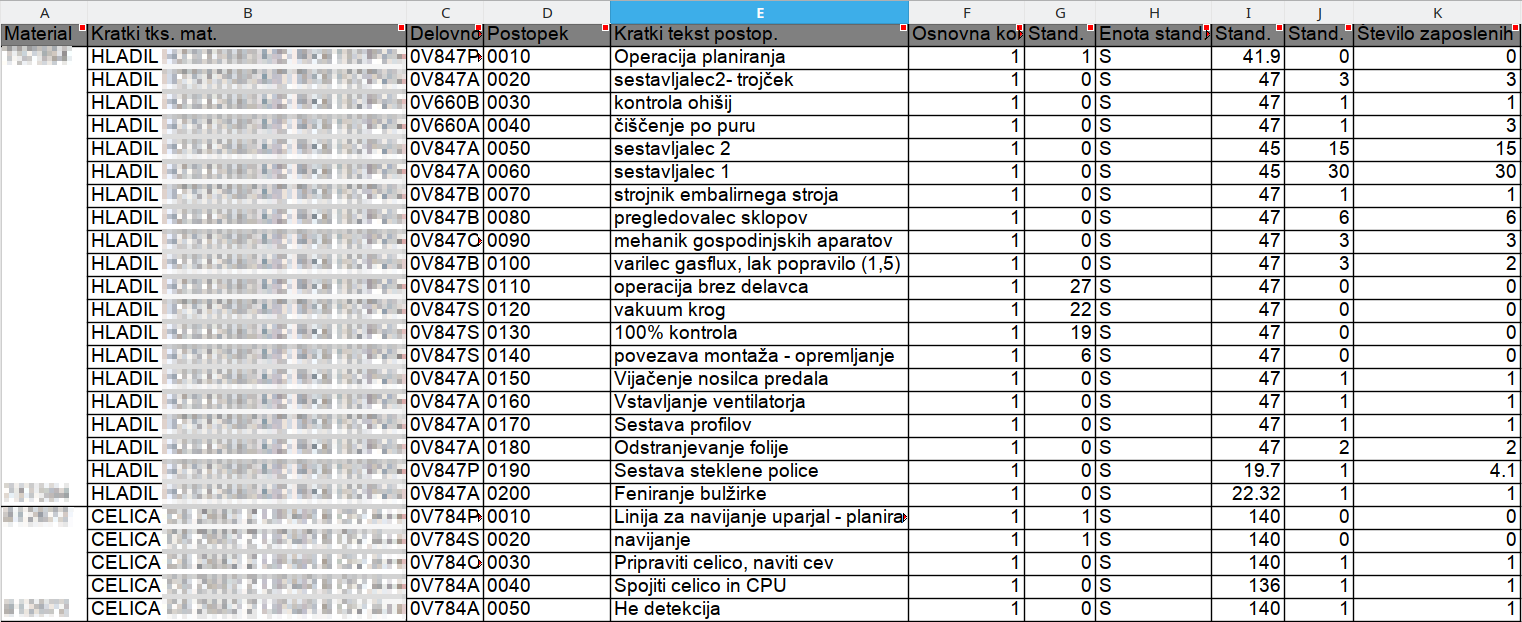
\includegraphics[width=11cm]{sap_2}
\end{center}
\caption{V tabelo izvožen opis tehnološkega postopka}
\label{sap_2}
\end{figure}

% Ta opis tehnološkega postopka je strukturiran tako, da se vsi koraki sklicujejo na eno samo tehnično sliko.

% // kako podrobno se opisuje korake?

\subsection{Definicija hipoteze}

V tej diplomski nalogi raziščemo nekaj trenutnih metod izdelave opisa tehnološkega postopka.
Raziskati želimo prednosti in slabosti trenutnih metod za izdelavo teh dokumentov.
V naslednji fazi raziskave želimo izdelati specializiran sistem za pisanje opisov tehnoloških postopkov.
Raziskati želimo, ali uporaba glasovnega asistenta v takšnem sistemu skrajša interakcije z mobilno aplikacijo.

Izhajajoč iz navedenega opredeljujem hipotezo diplomskega dela: Proces izdelave opisa tehnološkega postopka lahko naredimo učinkovitejši z uporabo glasovnega asistenta Amazon Alexa.

Potrjena hipoteza bi dokazovala visoko zrelost tehologije Amazon Alexa in dokazovala možnost uporabe v naprednih situacijah.

\section{Analiza obstoječih rešitev}

\subsection{Papir in pisalo}

Najstarejša metoda za izdelavo takšnega dokumenta je zapis na formuliran list papirja (// citiraj sliko).

// slika delavniškega dnevnika na papirju

Prednosti uporabe papirja in pisala so, da pri delu izdelovalec ne potrebuje računalnika in cenovna ugodnost.
Slabosti takšnega postopka so:
\begin{itemize}
	\item omejitve glede velikosti prostora, namenjenega vsakemu koraku,
	\item problematično dopisovanje in urejanje obstoječih korakov,
	\item rokopis je lahko nečitljiv,
	\item zahtevnejše arhiviranje, kot računalniške datoteke,
	\item občutljivost papirja na fizične poškodbe (trganje, mečkanje, vnetljivost,...).
\end{itemize}

// slika testni primer za čiščenje tipkovnice na papirju

\subsection{Pisarniški programi}

Opis tehnološkega postopka lahko izdelamo v pisarniških programih kot so Microsoft Word ali LibreOffice Writer.

Ta pristop reši večino slabosti uporabe papirja in pisala za pisanje opisa tehnološkega postopka.
Korake lahko enostavno dodajamo in urejamo.
Prav tako je možno dodajati slikovno gradivo.
Pisarniški programi omogočajo tudi enostaven izvoz dokumenta na tiskalnik, če želimo imeti dokument na listu papirja.

Prednost pisarniških programov je tudi možnost uporabe računalniške tipkovnice za vnos besedila.

Kljub temu pa uporaba te metode prinese nove slabosti:
\begin{itemize}
	\item če imamo dokument na več mestih, moramo ob spremembah zagotoviti, da se spremenijo vsi.
	\item Slikovno gradivo je vezano na dokument. Ob spremembah moramo spremeniti celoten dokument, ne le slike.
	\item Možnost izgube ali izbrisa podatkov.
\end{itemize}

V sklopu te diplomske naloge smo se odločili napisati preprost opis tehnološkega postopka (Slika \ref{report_writer}) s programom LibreOffice Writer \cite{writer}.
Pisanje in urejanje dokumenta je trajalo 10 minut.
Enostavno ga je bilo izvoziti v format PDF.
Dokument brez vsebine se lahko pri naslednjem opisu uporabi kot šablona.

\begin{figure}[H]
\begin{center}
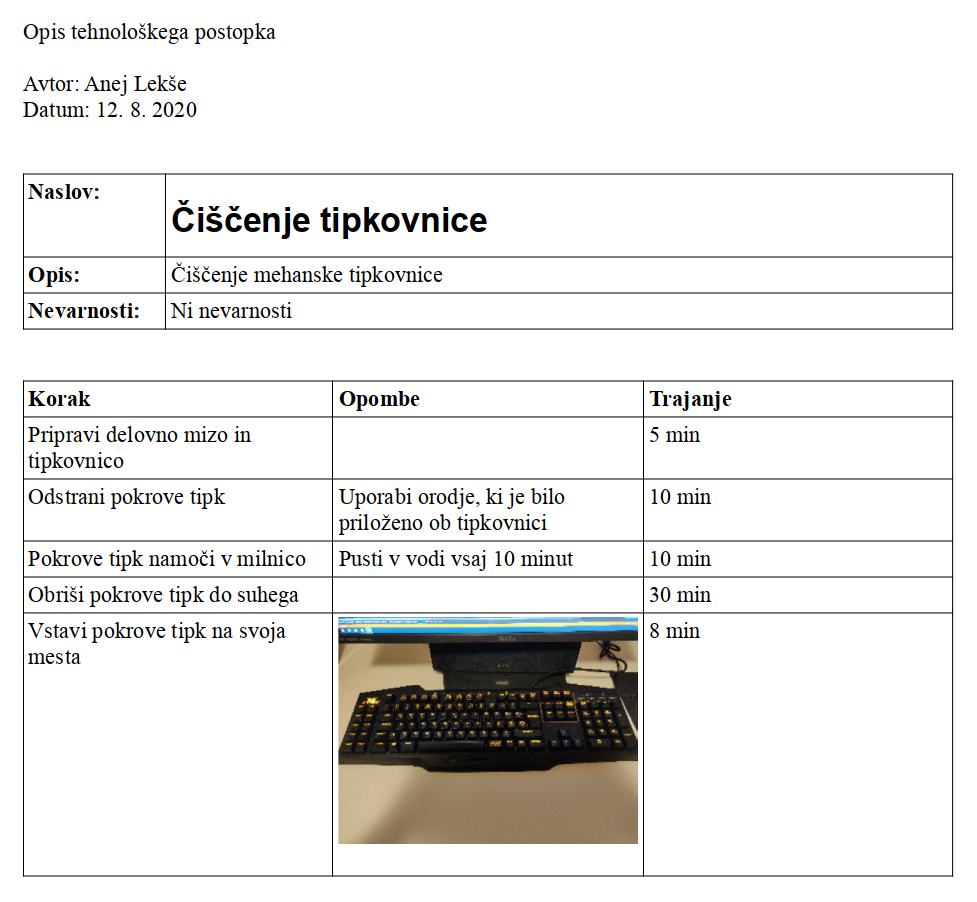
\includegraphics[width=11cm]{report_writer}
\end{center}
\caption{Preprost opis tehnološkega postopka v pisarniškem programu}
\label{report_writer}
\end{figure}

\subsection{Specializirani moduli za poslovne informacijske sisteme}

Podjetja in tovarne za svoje izdelke večinoma uporabljajo specializirane module, tesno povezavne z njihovimi informacijskimi sistemi.
Primer je prikazan modul za informacijski sistem SAP (Slika \ref{sap_1}).

\begin{figure}[H]
\begin{center}
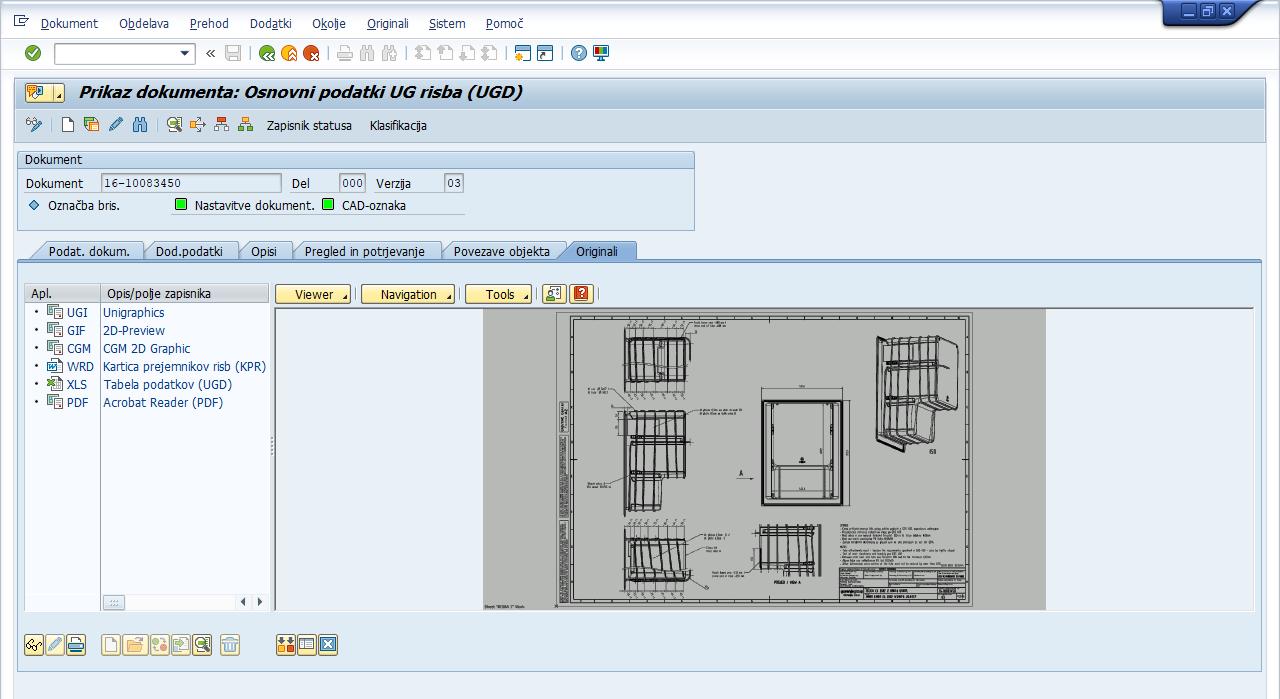
\includegraphics[width=13cm]{sap_1}
\end{center}
\caption{Prikazan korak opisa tehnološkega postopka s programom SAP}
\label{sap_1}
\end{figure}

Do tega opisa tehnološkega postopka se lahko dostopa iz računalnikov na delovnih mestih, kjer se izvajajo koraki, opisani v dokumentu.
Opis tehnološkega postopka v tem primeru sestavljajo:
\begin{itemize}
	\item podatki o izdelku,
	\item dodatne opombe,
	\item opisi korakov,
	\item definicija kontrolnih postopkov in pregleda, 
	\item CAD izris izdelka.
\end{itemize}

Specializiran informacijski sistem, kot je SAP, je tesno povezan s proizvodno linijo in prilagodljiv za potrebe proizvodnega obrata, ki ga uporablja.
Pri sistemu SAP se podatki primarno hranijo na centralnem strežniku, varnostna kopija pa se inkrementalno dela na geografsko ločen rezervrni strežnik.
Glavne slabosti takšnega sistema so:
\begin{itemize}
	\item potrebna proizvodna infrastruktura, ki jo sistem rabi za optimalen izkoristek in
	\item cena, ki je potrebna za implementacijo.
\end{itemize}

% V kemijski industriji se laboratorijska poročila pišejo s pomočjo LIMS (Laboratory Information Management System).
% Sistemi kot so OpenLIMS (// citiraj) imajo že vključene module za pisanje poročil (// citiraj)

% // testiraj LIMS 


\chapter{Načrtovanje in razvoj sistema za pisanje opisov tehnoloških postopkov}

\section{Definicija funkcionalnosti}

% Na podlagi raziskave obstoječih možnosti pisanja opisov tehnoloških postopkov smo definirali 
Pri načrtovanju sistema za pisanje opisov tehnoloških postopkov smo se osredotočali predvsem na nasledje točke:
% Učinkovit sistem za pisanje opisa tehnološkega postopka:
\begin{itemize}
	\item prekinitve dela, ki jih povzroči uporaba sistema morajo biti čim krajše,
	\item komponente sistema morajo biti enostavno zamenljive,
	\item uporabljene podatke (fotografije, zapiske) se mora hraniti na enem mestu.
	\item sistem mora biti popolnoma funkcionalen brez glasovnega asistenta.
\end{itemize}

% Sistem, ki ga bomo sprogramirali v tej raziskavi bo namenjen predvsem individualnim uporabnikom in bo mišljen kot alternativa pisanju delavniških dnevnikov na list papirja ali s pisarniškimi programi.
Sistem, ki ga bomo sprogramirali v tej raziskavi služi kot primer kompleksnejšega sistema, katerga uporabo bi radi pospešili z uporabo glasovnega asistenta.

Sistem bo služil kot alternativni pristop k pisanju opisov tehnoloških postopkov z pisarniškimi programi.
Sistem mora podpirati ustvarjanje novega opisa tehnološkega postopka in odpiranje ter urejanje že ustvarjenih opisov tehnološkega postopka.

Vsak opis tehnološkega postopka mora imeti naslov, opis, seznam možnih nevarnosti pri delu in seznam korakov dela.

Seznam korakov dela mora podpirati dodajanje novih korakov, urejanje obstoječih korakov, brisanje obstoječih korakov in spreminjanje vrstnega reda korakov.

Glasovni asistent bo imel naslednje vloge:
\begin{itemize}
	\item za trenutno odprt opis tehnološkega postopka bo z njim možno dodajati korake postopka,
	\item z njim bo možno odpreti kamero ali obrazec za dodajanje koraka.
\end{itemize}

Raziskava iz leta 2018 je pokazala izboljšano učinkovitost pri delu raziskovalcev v kemijskem laboratoriju, v katerega so integrirali glasovne pomočnike \cite{austerjost2018introducing}.
Namen raziskave je bil preizkus praktične uporabnosti glasovnih asistentov za branje laboratorijskih postopkov po korakih in glasovno upravljanje laboratorijskih instrumentov.
Pozitivni rezultati bi lahko bili ključnega pomena za slabovidne člane laboratorijev.
Kot glasovni asistent je bila uporabljena Amazon Alexa.
Prepoznavanje govora in ukazov je bilo konsistentno in hitro, ne glede na spol uporabnika.
Motnje pri razpoznavanju je povzročal večinoma ozadni hrup.
Povprečna natančnost prepoznave ukazov je bila 95\%.
Raziskovalci so zabeležili tudi problem moteče kakofonije v laboratoriju, v katerem je več raziskovalcev, ki uporabljajo glasovni nadzor naprav.

\section{Načrt}

Sistem za pisanje opisov tehnoloških postopkov smo poimenovali OpenReport. 
Sistem OpenReport bodo sestavljali:

\begin{itemize}
	\item strežniški program, 
	\item mobilna aplikacija,
	\item glasovni asistent.
\end{itemize}

Strežnik bo v podatkovni bazi hranil uporabnike, delavniške dnevnike in korake.
Uporabnik bo lahko do podatkov na strežniku dostopal preko mobilne aplikacije.
Glasovni asistent bomo uporabili kot komplement mobilne aplikacije.
Omogočal bo glasovno upravljanje aplikacije in narekovanje korakov.

\noindent Preko mobilne aplikacije bo uporabnik lahko:
\begin{itemize}
	\item opravil regsitracijo in prijavo,
	\item ustvaril nov delavniški dnevnik,
	\item odprl obstoječe delavniške dnevnike,
	\item ustvaril in urejal korake delavniškega dnevnika,
	\item zajemal slike in jih vstavljal v delavniški dnevnik,
	\item brisal korake delavniškega dnevnika,
	\item urejal vrstni red korakov delavniškega dnevnika.
\end{itemize}

Za glasovni asistent Amazon Alexa bomo razvili ''Skill'', s katerim bo uporabnik lahko:

\begin{itemize}
	\item v odprto poročilo vstavil dobesedno narekovan korak,
	\item odprl obrazec za dodajanje novega tekstovnega koraka,
	\item odprl kamero in obrazec za dodajanje koraka s fotografijo.
\end{itemize}

\begin{figure}[H]
\begin{center}
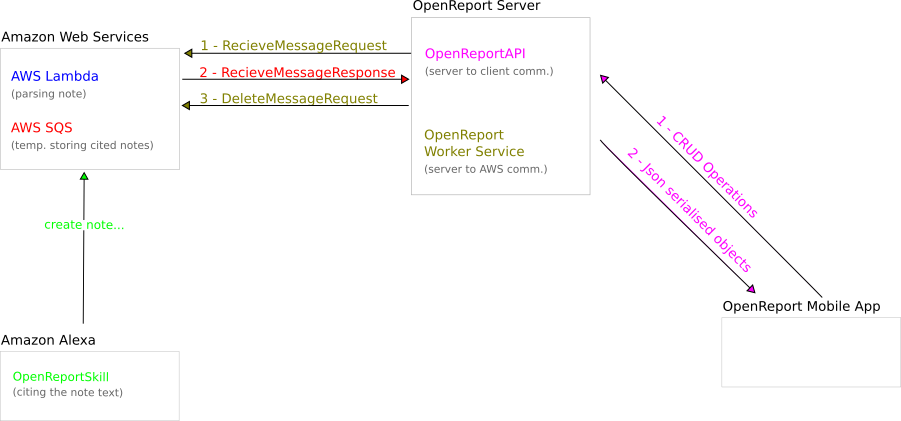
\includegraphics[width=13cm]{plan}
\end{center}
\caption{Visokonivojski načrt sistema}
\label{plan}
\end{figure}

\subsection{Zasnova aplikacije in vpliv na hipotezo}

Mobilna aplikacija bo služila kot primaren način za interakcijo s strežnikom.

V tej diplomski nalogi raziskujemo, ali je možno z vpeljavo glasovnega asistenta v naš sistem izboljšati učinkovitost tega sistema.
Da bodo rezultati raziskave čim bolj natančni, bomo dali učinkovitosti mobilne aplikacije velik poudarek.
Uporabniški vmesnik bo zasnovan za čim hitrejše delo.
To nam bo v zagotovilo, da uporabniški vmesnik aplikacije ni ''ozko grlo'' pri pisanju opisov tehnoloških postopkov.

Če bo delo z aplikacijo kljub dodelanemu in učinkovitemu uporabniškemu vmesniku hitrejše, bomo hipotezo potrdili.
V nasprotnem primeru bomo hipotezo ovrgli.

\section{Uporabljene tehnologije in programska oprema}

\subsection{.NET}

.NET je razvojna platforma, razvita s strani Microsofta.
Obsega programske jezike, prevajalnike, orodja in knjižnice, ki omogočajo širok spekter primerov uporabnosti, hkrati pa se ohranja enovitost ozadne kode.

Tehnologije .NET ogrodja, ki smo jih uporabil v tej diplomski nalogi so:
\begin{itemize}
	\item .NET Core - odprtokodna platforma za razvoj spletnih storitev,
	\item Xamarin, ki je ogrodje za razvoj mobilnih aplikacij za najpogostejše mobilne operacijske sisteme (Android, iOS).
\end{itemize}

.NET smo izbrali, saj je zelo dobro integriran z Amazonovim AWS API-jem in je dobro dokumentiran.

\subsection{Xamarin}

Ogrodje Xamarin \cite{xamarin} je odprtokodno orodje za razvoj mobilnih aplikacij, ki ga je razvil Microsoft. 

Z ogrodjem Xamarin je mogoče pri deliti večino ozadne in ospredne kode med različnimi mobilnimi operacijskimi sistemi. 
Za ozadno kodo se uporablja .NET (C\#), za front-end pa se uporablja XAML (Extensible Application Markup Language).

Xamarin smo izbral, da bomo lahko strežniški program in mobilno aplikacijo programirali v enakem programskem jeziku (C\#).

\subsection{Amazon Alexa}

Amazon Alexa je glasovni asistent, razvit s strani podjetja Amazon \cite{alexa}.
Za Amazon Alexo smo se odločili, saj ponuja enostavno možnost programiranja s ''Skill-i''.
Poleg tega je Alexo enostavno integrirati z drugimi Amazonovimi spletnimi storitvami, ki jih bomo uporabili v tej diplomski nalogi (AWS SQS, AWS Lambda).

\subsection{Alexa Skill}

Alexine osnovne funkcionalnosti lahko nadgradimo s programi, ki se jim reče ''Skill'' \cite{alexaskills}.
Da lahko ustvarimo in objavimo ''Skill'' rabimo račun Amazon razvijalca (\textit{ang. Amazon Developer Account}).


\noindent ''Skill'' sestavljajo:
\begin{itemize}
	\item \textbf{Invocation} - fraza, ki ''Skill'' zažene,
	\item \textbf{Intent} - fraze, ki jih ''Skill'' razpozna kot funkcije,
	\item \textbf{Endpoint} - omrežni vir, kjer se nahaja ozadna koda ''Skill-a''.
\end{itemize}

Ko Alexa zasliši ''Invocation'' ali katerega od ''Intent-ov'', glasovni posnetek pošlje na Amazonov strežnik.
Ta s pomočjo glasovnega razpoznavnega modela prepozna ukaze in pošlje poseben zahtevek na ''Endpoint''.
To je lahko druga Amazonova storitev (npr. AWS Lambda), storitev na Microsoftovem Azure strežniku ali naš lasten strežnik, dostopen preko javne domene.

Ko ''Endpoint'' obdela zahtevo, se odgovor pošlje nazaj na Amazonov strežnik v obliki znakovnega niza.
Ta podatek se nato pošlje nazaj na uporabnikovo Alexo, ki prejeti znakovni niz ''izgovori''.

\subsection{Amazon Web Services}

AWS je skupek oblačnih storitev, ki jih ponuja podjetje Amazon.
Ponuja integracijo s pogostimi programskimi jeziki in ogrodji, kot so Java, .NET, Python in Node.js preko storitve AWS API.
Pri tej diplomski nalogi smo se osredotočili na dva sistema iz skupka AWS.

\subsubsection{AWS SQS}

AWS SQS je sistem za pošiljanje tekstovnih sporočil med odjemalci preko Amazonovih strežnikov \cite{sqs}.
Za hranjenje sporočil je treba registrirati ''SQS Queue'' \textit{(slo. SQS vrsto)}. 
Ta je lahko neurejena vrsta, kjer prejeta sporočila niso nujno urejena po času ustvarjanja, lahko pa je tipa FIFO, pri kateri je zagotovljeno, da dobimo vsa sporočila v vrstnem redu, v katerem so bila poslana.
V sklopu te diplome smo uporabili vrsto FIFO.

To storitev bomo uporabili za komunikacijo med Amazon Alexo in OpenReport strežnikom.

\subsubsection{AWS Lambda}

Ozadno kodo za Alexa ''Skill'' smo gostili na platformi AWS Lambda.
To je storitev za gostovanje dogodkovno vodene ozadne kode \cite{lambda}.
Za to platformo smo se odločili zaradi dobre integracije z ''Alexa Skill Kit-om'' in razvojnim orodjem Visual Studio.

\section{Strežnik}

Za uporabo centralnega strežnika smo se odločili, da lahko do hranjenih podatkov dostopamo iz različnih naprav preko enotnega vmesnika (API).
V našem primeru bosta s strežnikom komunicirala mobilna aplikacija in glasovni asistent.
Podatke bomo hranili v podatkovni bazi, ki jo streže SQL Server.

Baza hrani tabele ''Users'' (\textit{slo. Uporabniki}), ''Projects'' (\textit{slo. Projekti}) in ''Notes'' (\textit{slo. Zapiski}) (Slika \ref{er_diagram}).
Vsak uporabnik lahko ima 0 ali mnogo projektov (opisov tehnološkega postopka).
Vsak projekt ima lahko 0 ali mnogo zapiskov (korakov).

\begin{figure}[H]
\begin{center}
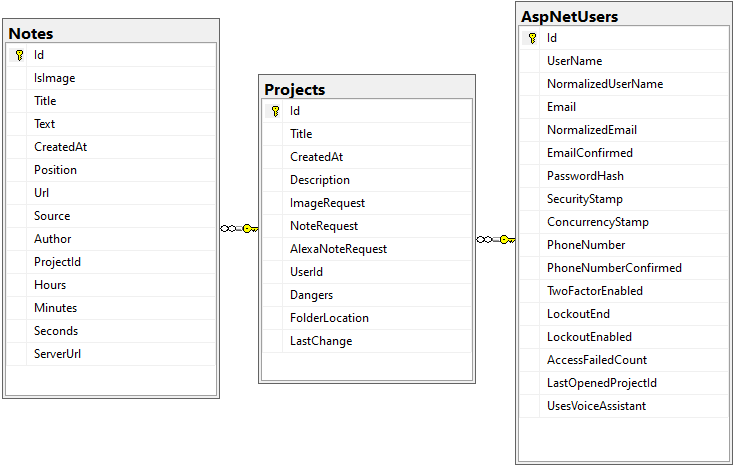
\includegraphics[width=11cm]{er_diagram_small}
\end{center}
\caption{ER model podatkovne baze}
\label{er_diagram}
\end{figure}

% // bom resizal in iz slike odstranil tabele, ki jih ne rabimo

\noindent Strežnik ima naslednje naloge:
\begin{enumerate}
	\item komunikacija s podatkovno bazo,
	\item komunikacija z odjemalcem (mobilno aplikacijo),
	\item komunikacija z glasovnim asistentom (Amazon Alexa),
	\item ponujanje vmesnika, preko katerega lahko odjemalci delajo s podatki v bazi.
\end{enumerate}


\subsection{Implementacija API}

Komunikacija med strežnikom in odjemalci poteka preko HTTP po pristopu API.
Podatki se prenašajo v formatu JSON.
To metodo smo izbrali zaradi enostavnosti implementacije in možnosti širjenja nabora klientov v prihodnosti.

Ker lahko sistem uporablja več uporabnikov, smo se odločili implementirati sistema za avtentikacijo uporabnikov in avtorizacijo zahtev.
Avtentikacija z uporabniškim imenom in geslom omogoča preverjanje identitete.
Ko se vzpostavi zaupanje, se prijavljenemu uporabniku dodeli avtorizacijski žeton.
Iz žetona je možno razbrati, za katerega uporabnika gre in katere pravice so mu dodeljene.

\subsubsection{Registracija in prijava}

Pri registraciji mora odjemalec poslati na API objekt razreda \textit{RegisterUserRequest}.
Odjemalec ga mora poslati na URL ''\texttt{/identity/register}''.

\begin{verbatim}
RegisterUserRequest {
    string Email; 
    string Password; 
} 
\end{verbatim}


Ko strežnik prejme ta objekt, ga pošlje v avtentikacijsko storitev.
V tej storitvi preveri, ali uporabnik s tem uporabniškim imenom že obstaja.
Če obstaja, se zabeleži napaka in nadaljnja registracija se prekine.
Če ta uporabnik ne obstaja, se kreira nov objekt razreda \texttt{User}.
Polje \texttt{Password} se zakriptira in se skupaj s poljem \texttt{Email} zapiše v ta objekt.
Uporabnik pa pri registraciji dobi tudi svoj unikaten identifikator \texttt{UserID}.

V kolikor se je v avtentikacijski storitvi dogodila kakršna koli napaka, se klientu vrne objekt razreda \texttt{AuthFailedResponse}

\begin{verbatim}
AuthFailedResponse { 
     IEnumerable<string> Errors; 
}
\end{verbatim}

\noindent V tem objektu se odjemalcu v zbirki pošljejo vse napake, ki jih je avtentikacijska storitev zabeležila pri neuspešni registraciji. 
Če je bila registracija uspešna, se odjemalcu pošlje objekt razreda \texttt{AuthSuccessResponse}

\begin{verbatim}
AuthSuccessResponse { 
    string UserId; 
    string Token; 
} 
\end{verbatim}

\noindent V polje \texttt{Token} se zapiše avtorizacijski žeton.
Žeton je tipa JWT ali \textit{JSON Web Token}.
Sestavljajo ga e-mail uporabnika, uporabnikov unikatni identifikator \texttt{UserID}, čas zapada žetona in tip simetričnega kodiranja, uporabljenega za enkripcijo žetona.

Objekt \texttt{AuthSuccessResponse} se nato pošlje nazaj odjemalcu.
Odjemalec nato žeton iz prejetega objekta doda glavi vseh svojih HTTP zahtevkov na OpenReport strežnik.
V nadaljnji komunikaciji, strežnik iz žetona razbere uporabnikov unikatni identifikator in ga uporabi pri poizvedbah po podatkovni bazi.

Prijava poteka podobno.
Uporabnik mora poslati na strežnik objekt \textit{LoginUserRequest}.
URL, na katerega mora odjemalec preko POST metode poslati ta objekt, je ''\texttt{/identity/login}''.

\begin{verbatim}
LoginUserRequest {
    string Email; 
    string Password; 
} 
\end{verbatim}

Ko strežnik prejme ta objekt, ga pošlje v avtentikacijsko storitev.
V tej storitvi preveri, ali uporabnik že obstaja.
Če ta uporabnik ne obstaja, ali pa je njegovo zakriptirano geslo v podatkovni bazi drugačno kot to, kar je v polju \texttt{Password}, se zabeležijo napake in prijava se prekine.
Odjemalec prejme objekt razreda \texttt{AuthFailedResponse}.

Če uporabnik obstaja in se njegovo zakriptirano geslo iz polja \texttt{Password} ujema z geslom v podatkovni bazi, je avtentikacija uspešna.
Odjemalec prejme objekt razreda \texttt{AuthFailedResponse}.

V primeru uspešne avtentikacije se avtorizacijski žeton \texttt{Token} generira in pošlje enako kot pri registraciji.

\subsubsection{Operacije z delavniškimi dnevniki}

Vsak uporabnik lahko ima nič ali več delavniških dnevnikov.

Vse operacije nad uporabnikovim delavniškim dnevnikom morajo biti avtorizirane.
V kolikor niso, bo API vedno javil napako \texttt{Bad Request: Not Authorised}.

Pri ustvarjanju novega opisa tehnološkega postopka (v nadaljevanju poglavja \textit{projekta}) mora uporabnik podati naslov, kratek opis projekta in seznam možnih nevarnosti.

To odjemalec zapiše v objekt razreda \texttt{CreateProjectRequest}.

\begin{verbatim}
CreateProjectRequest { 
    string Title;  
    string Description; 
    string Dangers; 
} 
\end{verbatim}

\noindent Ta objekt se nato pošlje preko POST metode na strežnik na naslov \texttt{/projects/create}.
Storitev za operacije nad projekti nato kreira nov objekt razreda \texttt{Project} s podatki iz prejete zahteve.
V primeru, da je zahteva ustrezno formulirana in avtorizirana, se projekt zapiše v podatkovno bazo.
Odjemalcu se kot odgovor pošlje ustvarjen objekt tega projekta.

\noindent Razred \texttt{Project} izgleda tako:

\begin{verbatim}
Project { 
    int Id; // unikatni identifikator 
    string Title; 
    string Description; 
    string Dangers; 
    IEnumerable<Note> Notes; // seznam korakov 
    ... 
}
\end{verbatim}
Do kateregakoli svojega projekta lahko odjemalec v nadaljnji komunikaciji dostopa tako, da pošlje GET zahtevek na URL ''\texttt{/projects/\{id\}}''.
Polje \texttt{\{id\}} mora v tem primeru biti unikatni identifikator projekta.

Za izbris projekta mora uporabnik poslati DELETE zahtevo na URL ''\texttt{/projects/\{id\}}''.
Če zahteva ni avtorizirana z ustreznim žetonom, se projekt ne izbriše.

\subsubsection{Operacije nad koraki opisa tehnološkega postopka}

Vsak projekt ima lahko nič ali več korakov.
Vsak korak ima naslov, opis in predvideno trajanje.

Korak je lahko izključno tekstovni, lahko pa ima tudi pripadajočo sliko.

Da ustvarimo tekstovni korak moramo poslati objekt razreda \texttt{Note} preko POST metode na URL ''\texttt{/projects/\{id\}/addnote}''.
Polje \texttt{\{id\}} mora biti unikatni identifikator projekta, katermu želimo dodati korak.

\noindent Razred \texttt{Note} izgleda tako.

\begin{verbatim}
Note { 
    ... 
    string Title; 
    string Text; 
    int Hours; 
    int Minutes;
    int Seconds;
    ...
}
\end{verbatim}

Strežnik najprej preveri, če je pošiljatelj poslal avtorizirano zahtevo.
Iz avtorizacijskega žetona strežnik razbere uporabnikov \texttt{UserID}. 
Če je projekt z identifikatorjem \texttt{id} res v lasti uporabnika z identifikatorjem \texttt{UserID}, se bo korak dodal v zbirko korakov tega projekta.

Če želimo ustvariti slikovni korak, moramo poslati objekt razreda \textit{UploadImageRequest} na URL ''\texttt{/projects/\{id\}/addimage}''.

\begin{verbatim}
UploadImageRequest { 
    Note note; 
    string ImageString; 
}
\end{verbatim}

V tem razredu predstavlja polje \texttt{ImageString} pripadajočo fotografijo, zakodirano v znakovni niz.
Za kodirni algoritem smo uporabili Base64.

Za hranjenje tekstovnih in slikovnih korakov smo zaradi preprostosti implementacije uporabili isti razred (\texttt{Note}).
Tekstovni in slikovni korak se ločita v vrednosti boolean zastavice \texttt{IsImage}.
Tekstovni korak ima to zastavico nastavljeno na vrednost \texttt{false}, slikovni pa \texttt{true}.

\begin{Verbatim}[commandchars=+\[\]]
Note { 
    +underline[bool IsImage;]
    string Title; 
    string Text; 
    int Hours; 
    int Minutes;
    int Seconds; 
    +underline[string Url;] // Lokacija slike na klientu
    +underline[string ServerUrl;] // Lokacija slike na strežniku
    ... 
}
\end{Verbatim}

Poljema \texttt{Url} in \texttt{ServerUrl} se dodeli vrednost samo pri slikovnih korakih.
Ko se na klientu zajame fotografija, klient nastavi vrednost polja \texttt{Url} na lokacijo ustvarjene fotografije v datotečnem sistemu.

Polje \texttt{ServerUrl} se nastavi šele na strežniku.
Ko strežnik prejme zahtevo za kreiranje slikovnega koraka, se korak \texttt{Note} prebere iz objekta \texttt{UploadImageRequest} in zapiše v podatkovno bazo.
Nato se \texttt{ImageString} dekodira in hrani na strežniku.
Ko se fotografija uspešno zapiše v datotečni sistem, se v polje \texttt{ServerUrl} zapiše lokacija pravkar ustvarjene datoteke na strežniku in spremembe se hranijo v podatkovni bazi.

\subsubsection{Urejanje in brisanje in korakov v projektu}

Da se korak v projektu izbriše, moramo poslati avtorizirano zahtevo na URL ''\texttt{/projects/\{pid\}/delete/\{nid\}}''.
V tem primeru je polje \texttt{\{pid\}} unikatni identifikator projekta, v katerem se nahaja korak, \texttt{\{nid\}} pa unikatni identifikator objekta \texttt{Note}, ki ga želimo izbrisati.
V kolikor ima ta objekt \texttt{Note} postavljeno zastavico \texttt{IsImage} na \texttt{true}, se poleg zapisa v bazi izbriše tudi pripadajoča slikovna datoteka.

Pri posodabljanju (urejanju) tekstovnih korakov, moramo poslati avtorizirano PUT zahtevo na URL ''\texttt{/projects/\{pid\}/update/\{nid\}}''.
Telo zahteve mora vsebovati objekt razreda \texttt{Note}.

Pri posodabljanju slikovnih korakov pošljemo avtorizirano PUT zahtevo na naslov ''\texttt{/projects/\{pid\}/update/\{nid\}/image}''.
Telo te zahteve mora vsebovati objekt razreda \texttt{UploadImageRequest}.
V temu objektu mora biti polje \texttt{Note} objekt, ki ga želimo posodobiti.
Polje \texttt{ImageString} mora biti, po metodi Base64, zakodirana slika, ki bo zamenjala prejšnjo sliko.

\subsubsection{Spreminjanje vrstnega reda korakov v projektu}

Položaj koraka \texttt{Note} v projektu lahko razberemo iz atributa \texttt{Position}.
Prvi korak ima \texttt{Position} 0, drugi 1, itd.

\begin{Verbatim}[commandchars=+\[\]]
Note { 
    int Id; 
    +underline[int Position;]
    bool IsImage;  
    string Title; 
    string Text;
    int Hours; 
    int Minutes;
    int Seconds;
    string Url;
    string ServerUrl;
}
\end{Verbatim}

Pri dodajanju korakov v projekt se obstoječe korake projekta razvrsti po vrednosti polja \texttt{Position}.
Vzamemo največjo vrednost tega polja in ji prištejemo 1.
Nato to vrednost priredimo polju \texttt{Position} novo kreiranega koraka.

Ko želimo spremeniti pozicijo koraka v projektu, moramo poslati zahtevo PUT na URL ''\texttt{/projects/\{pid\}/\{nid\}/\{positions\}}''.

V tem primeru je polje \texttt{\{pid\}} unikatni identifikator projekta, v katerem se nahaja korak, \texttt{\{nid\}} unikatni identifikator koraka \texttt{Note}, \texttt{Positions} pa število mest za kolikor ga želimo prestaviti.
To število je lahko pozitivno ali negativno celo število.
Negativna vrednost prestavi korak proti začetku seznama, pozitivna pa proti koncu.

\subsubsection{Izvoz projektov}

Projekt lahko izvozimo v dva formata, v tekstovno datoteko in HTML dokument.

To naredimo tako, da pošljemo avtorizirani GET zahtevi na URL-ja ''\texttt{/projects/\{id\}/export/text}'' ali ''\texttt{/projects/\{id\}/export/html}''.

Pri izvozu v tekstovno datoteko storitev za upravljanje projektov na strežniku ustvari novo tekstovno datoteko.
Najprej vanjo vpiše naslov in opis projekta ter možne nevarnosti pri delu.
Nato uredi korake po vrednosti stolpca \texttt{Position} in enega za drugim zapiše v datoteko.
Če je korak slikovni, se zapiše tudi lokacija pripadajoče fotografije.

Pri izvozu v HTML dokument (Slika \ref{export_html}) se naslov zapiše kot HTML naslov H1, opis kot naslov H2, in koraki kot HTML odstavki.
V HTML dokumentu lahko prikažemo poleg slikovnih korakov tudi slike same.

\begin{figure}[H]
\begin{center}
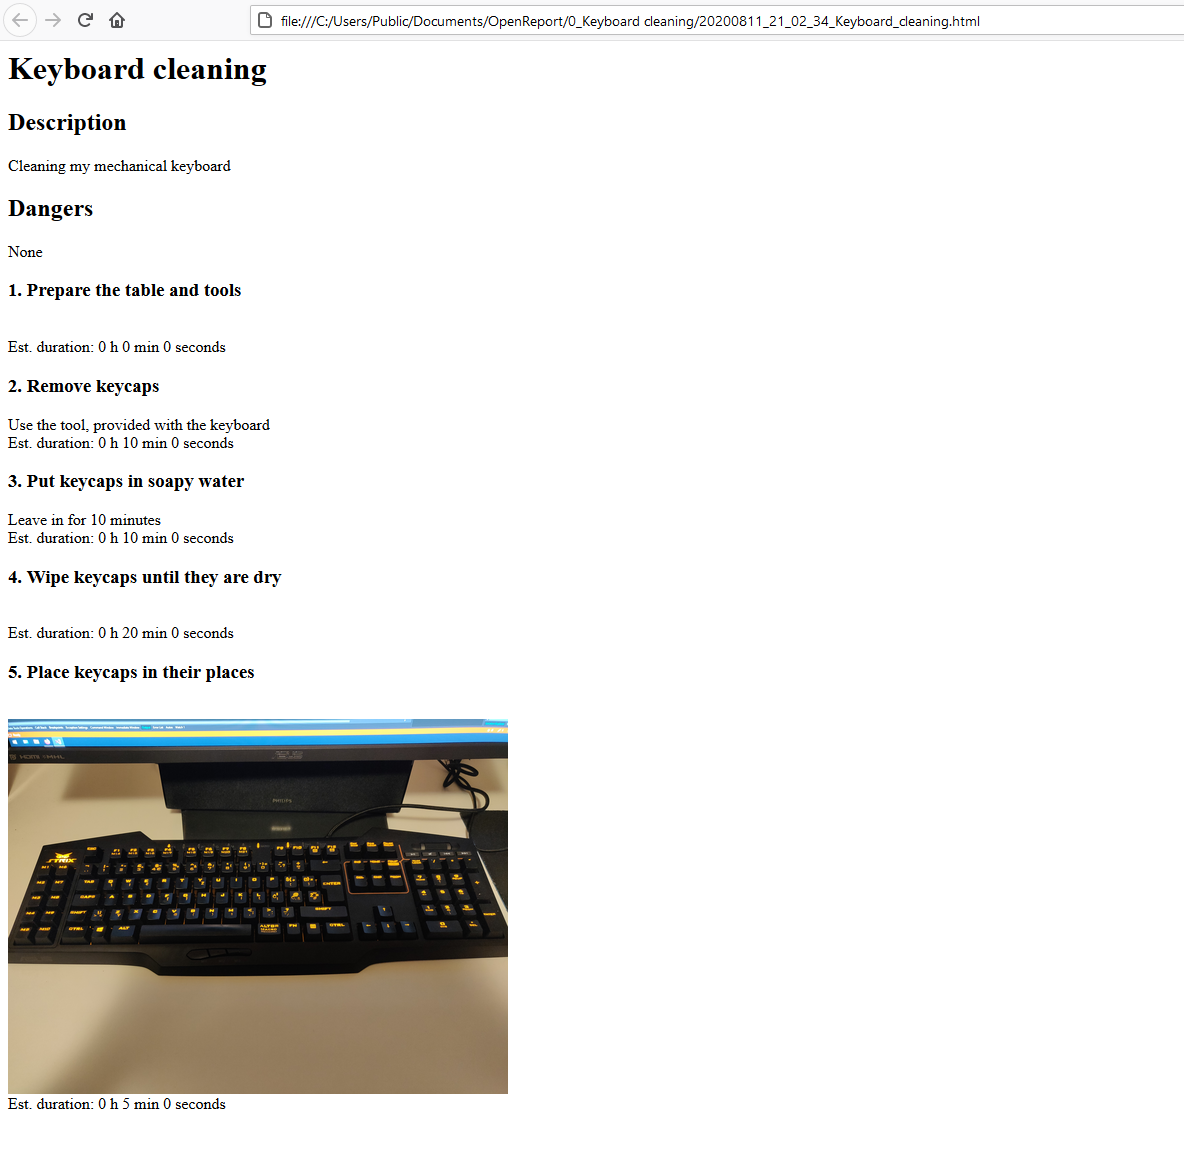
\includegraphics[width=13cm]{export_html}
\end{center}
\caption{Projekt, izvožen v HTML dokument}
\label{export_html}
\end{figure}

Lokacija izvožene datoteke se nahaja v polju \texttt{FolderLocation} v razredu \texttt{Project}.
Privzeta lokacija, ki se nastavi ob kreiranju projekta je 
\\''\texttt{C:/users/USER/Public Documents/OpenReport}''.

\begin{Verbatim}[commandchars=+\[\]]
Project {
    int Id; 
    string Title; 
    string Description; 
    string Dangers; 
    +underline[string FolderLocation;] // lokacija pripadajočih datotek 
    IEnumerable<Note> Notes; 
    ... 
}
\end{Verbatim}

\subsection{Komunikacija strežnika z glasovnim asistentom}

Strežnik z glasovnim asistentom Amazon Alexa komunicira preko storitve AWS SQS.
Glasovni asistent od uporabnika prejme glasovni ukaz.
Na podlagi tega ukaza lahko glasovni asistent na SQS vrsto odloži tri različna tekstovna sporočila:
\begin{itemize}
	\item \textbf{"addnote"},
	\item \textbf{"addimage"},
	\item \textbf{"\{narekovano besedilo\}"},
\end{itemize}

Sporočilo ''addnote'' sporoči strežniku, da naj odpre obrazec za dodajanje tekstovnega koraka.
Sporočilo ''addimage'' sporoči strežniku, da naj odpre kamero in obrazec za dodajanje slikovnega koraka.
Sporočilo ''\{narekovano besedilo\}'' sporoči strežniku, naj vsebino tega sporočila doda odprtemu projektu kot tekstovni korak.

\subsubsection{Utemeljitev uporabe SQS}
Za hranjenje sporočil v storitvi SQS smo se odločili po primerjavi z dvema alternativnima pristopoma.
Prvi je bil odpiranje omrežne vtičnice (ang. Web Socket).
Ta bi prinesla učinkovitejši prenos podatkov, implementacija pa bi bila težja.
Ta implementacija bi bila tudi manj prenosljiva, če bi menjal glasovnega asistenta.
Druga alternativa pa je bila direktna komunikacija Amazon Alexe in našega strežnika preko REST API zahtevkov, ki se prenašajo po protokolu HTTP.
Ta alternativa bi bila implementacijsko preprostejša kot uporaba SQS.
Problem te alternative bi bil, da bi bilo treba javno odpreti API dostopne točke, ki jih lahko asistent uporablja, ali implementirati nove metode za avtentikacijo in avtorizacijo zahtevkov iz glasovnega asistenta.

Uporaba SQS za hranjenje sporočil tudi omogoča enostavnejšo možnost zamenjave glasovnega asistenta.
Asistent, s katerim bi želeli zamenjati Amazon Alexo mora za dosego enake končne funkcionalnosti odložiti na SQS sporočila (''addnote'', ''addimage'',...) v pravem formatu.

\subsubsection{Zahtevanje in izpust glasovnega asistenta}

V sklopu našega projekta bomo na enem OpenReport strežniku uporabljali samo enega glasovnega asistenta.
Tega asistenta lahko uporabnik ''zahteva'' za lastno uporabo in ga po uporabi ''izpusti''.
Ali ima določen uporabnik nase vezanega asistenta, vidimo po vrednosti zastavice \texttt{UsesVoiceAssistant} v njegovem objektu razreda \texttt{User}.
Uporabnik asistenta uporablja, če je zastavica nastavljena na \texttt{True}.

Ko uporabnik odpre katerega od svojih projektov, se unikatni identifikator tega projekta nastavi v polje \texttt{LastOpenedProjectId} v njegovem objektu razreda \texttt{User}.

Zahtevki, ki jih strežnik prejme od glasovnega asistenta, se navezujejo na projekt s tem identifikatorjem.

\begin{Verbatim}[commandchars=+\[\]]
User : IdentityUser {
    string Id; 
    string Email;
    string Password; 
    IEnumerable<Project> Projects;
    ... 
    +underline[int LastUsedProjectId;]
    +underline[bool UsesVoiceAssistant;]
}
\end{Verbatim}

\subsubsection{Delovanje}

Na strežniku OpenReport teče storitev za komunikacijo z glasovnim asistentom.
Ta storitev vsakih deset sekund na SQS pošlje zahtevek \texttt{RecieveMessageRequest}.

\begin{Verbatim}[commandchars=+\[\]]
RecieveMessageRequest {
    AttributeName 
    MaxNumberOfMessages 
    QueueUrl 
    WaitTimeSeconds
    ... 
} 
\end{Verbatim}

AWS SQS kot odgovor vrne objekt tipa \texttt{RecieveMessageResponse}.

\begin{Verbatim}[commandchars=+\[\]]
RecieveMessageResponse {
    IEnumerable<Message> Messages;
    ...
}
\end{Verbatim}

V tem odgovoru se nahaja seznam sporočil, ki čakajo na sprejem iz SQS vrste.
V kolikor je v odgovoru vsaj eno sporočilo, pregledamo telo vseh sporočil. 

Ko sporočila sprejmemo, jih moramo izbrisati iz SQS vrste.
Če jih sproti ne izbrišemo, iz FIFO vrste ne moremo brati najnovejših sporočil, ampak le 5 najstarejših.

Sporočila izbrišemo iz vrste preko zahtevka \texttt{DeleteMessageRequest}.
Ta zahtevek hrani referenco na sporočilo, ki ga želimo izbrisati iz SQS vrste.
AWS SQS storitev v odgovor vrne \texttt{DeleteMessageResponse}, a v tej diplomski nalogi tega odgovora ne uporabljamo naprej.

Zahtevki, ki jih prejmemo od glasovnega asistenta v projektu, ki ga je uporabnik z glasovnim asistentom nazadnje odprl, nastavijo vrednosti treh boolean zastavic v objektu razreda \texttt{Project}.
\begin{itemize}
	\item Zahtevek ''\texttt{addnote}'' nastavi zastavico ''\texttt{NoteRequest}'' na \texttt{true},
	\item zahtevek ''\texttt{addimage}'' nastavi zastavico ''\texttt{ImageRequest}'' na \texttt{true},
	\item zahtevek ''\texttt{\{narekovano besedilo\}}'' nastavi zastavico ''\texttt{AlexaNoteRequest}'' na \texttt{true} in prejeto besedilo doda projektu kot korak.
\end{itemize}

\begin{Verbatim}[commandchars=+\[\]]
Project { 
    int Id; 
    string Title; 
    string Description; 
    string Dangers; 
    string FolderLocation; 
    IEnumerable<Note> Notes; 
    +underline[bool NoteRequest;] 
    +underline[bool ImageRequest;] 
    +underline[bool AlexaNoteRequest;] 
}
\end{Verbatim}


Če je vsebina prejetega sporočila enaka \texttt{addnote}, storitev preveri, kateri uporabnik ima trenutno nase vezanega glasovnega asistenta.
Nato v projektu, katerega je nazadnje odprl nastavi vrednost zastavice \texttt{NoteRequest} na \texttt{true}.


Če je vsebina enaka ''\texttt{addimage}'', storitev preveri, kateri uporabnik ima trenutno nase vezanega glasovnega asistenta.
Nato v projektu, katerega je nazadnje odprl nastavi vrednost zastavice \texttt{ImageRequest} na \texttt{true}.

Če vsebina prejetega sporočila ni enaka ''\texttt{addimage}'' ali ''\texttt{addnote}'', pomeni, da je prejeto sporočilo dobesedno narekovan korak.
Kot prej, storitev preveri, kateri uporabnik ima nase vezanega glasovnega asistenta.
Nato v projektu, katerega je nazadnje odprl nastavi vrednost zastavice \texttt{AlexaNoteRequest} na \texttt{true}.
Poleg tega ustvari nov objekt razreda \texttt{Note}, ki ima naslov ''Voice note'', vsebina pa je telo prejetega sporočila.
Nov objekt se nato vstavi v najden projekt.




\section{Implementacija ,,Alexa Skilla''}

Alexa ''Skill'' bomo uporabili za glasovno upravljanje aplikacije.
Glavni namen Alexa ''Skill-a'' v sklopu sistema OpenReport bo dodajanje korakov v opis tehnološkega postopka in odpiranje obrazcev za vstavljanje korakov.

\noindent Natančneje, ''Skill'' bo uporabniku omogočal:
\begin{itemize}
	\item dodajanje tekstovnega koraka,
	\item odpiranje kamere in dodajanje slikovnega koraka in
	\item dobesedno narekovanje besedila tekstovnega koraka.
\end{itemize}

Ko bo Alexa zaslišala ukaz za zagon ''Skill-a'' (ang. Invocation), se bo ''Skill'' začel izvajati.
Invokacijska fraza se glasi ''\textit{make a report note}''.

Vsak nadaljnji ukaz, ki ga bo uporabnik izrekel, preden se ''Skill'' preneha izvajati, se bo primerjal s frazami za zagon podprogramov ''Skill-a''.
Te fraze se imenujejo ''namere'' (ang. Intent).
V našem skillu bomo imeli tri glavne namere:

\begin{itemize}
	\item \texttt{TakeNoteIntent},
	\item \texttt{OpenTextNoteFormIntent},
	\item \texttt{OpenImageNoteFormIntent}.
\end{itemize}

\texttt{TakeNoteIntent} (Slika \ref{TakeNoteIntent}) se bo zagnal, ko bo po invokacijski frazi uporabnik izrekel ''\texttt{take note \{besedilo\}}'' ali ''\texttt{note \{besedilo\}}''.
Polje \texttt{\{besedilo\}} je tekstovna spremenljivka, v katero ''Skill'' hrani razpoznano tekstovno vsebino koraka.
V primeru, da uporabnik izreče ''\textit{note unscrew the backplate}'', bo vrednost spremenljivke \texttt{\{besedilo\}} ''unscrew the backplate''.

\begin{figure}[H]
\begin{center}
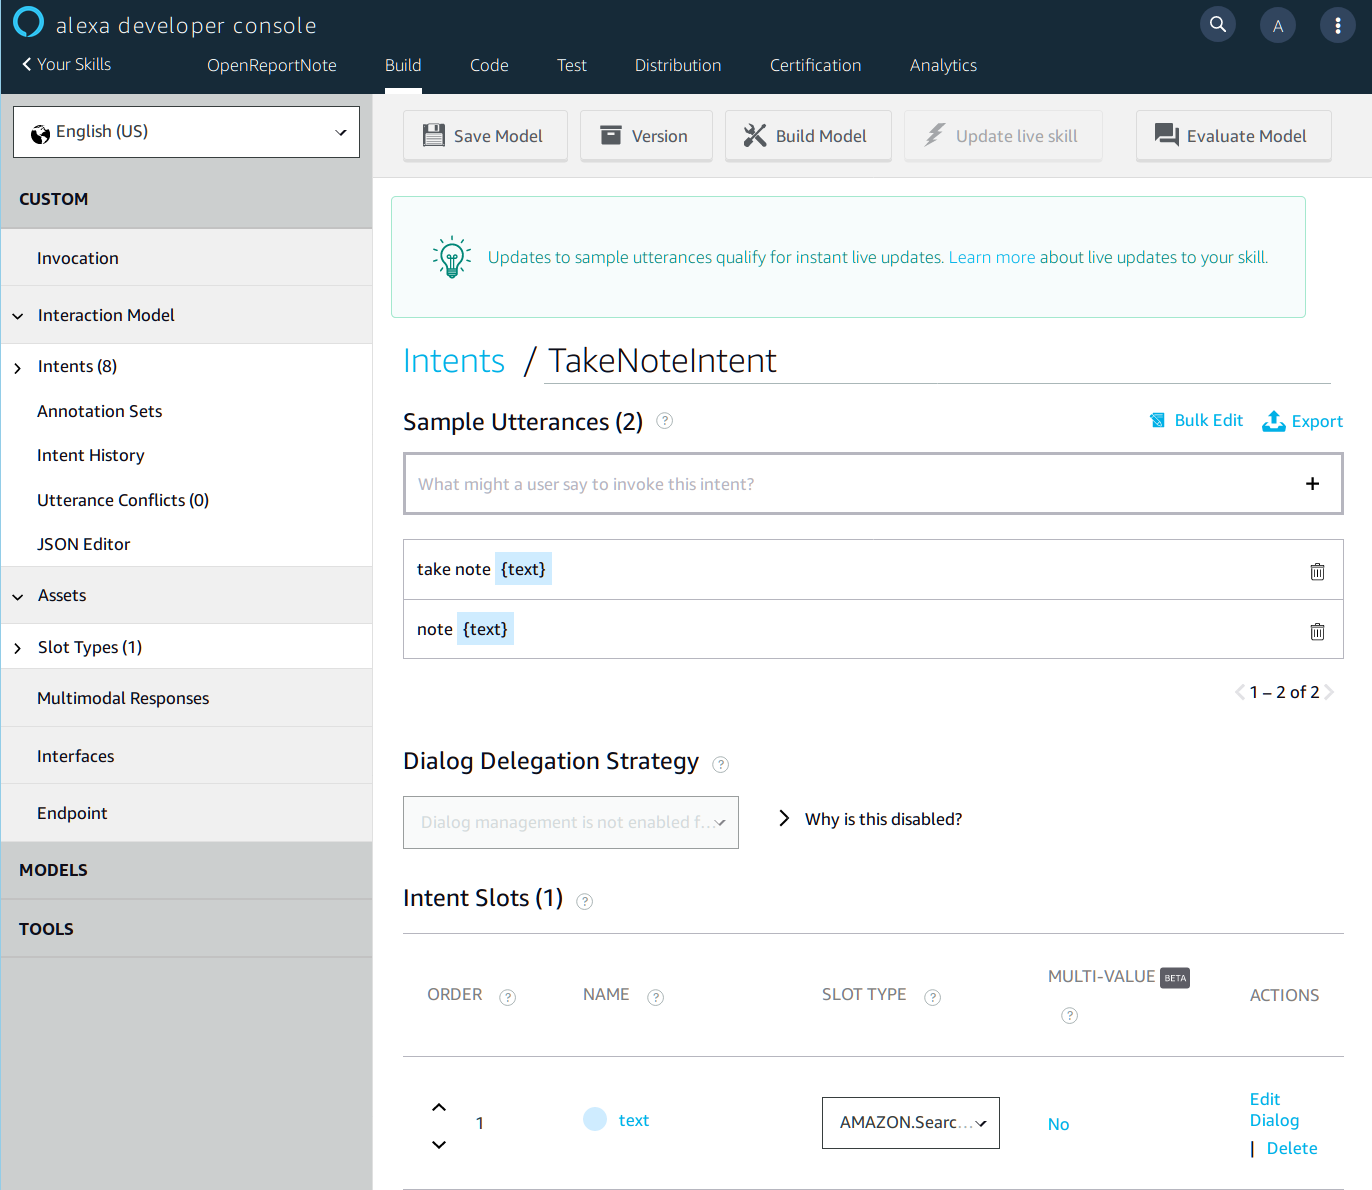
\includegraphics[width=13cm]{intent_literal}
\end{center}
\caption{TakeNoteIntent v Alexa Developer nadzorni plošči}
\label{TakeNoteIntent}
\end{figure}

Ta ''Intent'' bo v ozadni kodi ''Skill-a'' zagnal funkcijo, ki bo ustvarila novo SQS sporočilo.
V telo tega sporočila bo funkcija vstavila vrednost spremenljivke \texttt{\{besedilo\}} in ga poslala v SQS vrsto.
''Skill'' zatem vrne uporabniku odgovor ''Noted!'' in se preneha izvajati.

\texttt{OpenTextNoteFormIntent} se bo zagnal, ko bo po invokacijski frazi uporabnik izrekel ''\texttt{create a text note}''.

Ta ''Intent'' bo v ozadni kodi ''Skill-a'' zagnal funkcijo, ki bo ustvarila novo SQS sporočilo.
V telo tega sporočila bo funkcija vstavila vrednost ''\texttt{addnote}'' in ga poslala v SQS vrsto.
''Skill'' zatem vrne uporabniku odgovor ''Opening the form!'' in se preneha izvajati.


\begin{figure}[H]
\begin{center}
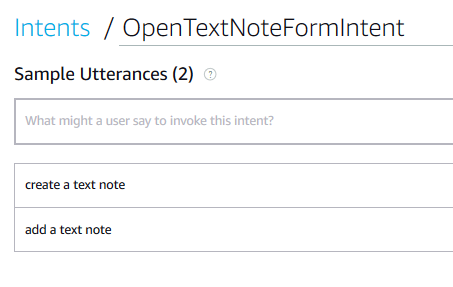
\includegraphics[width=8cm]{intent_text}
\end{center}
\caption{OpenTextNoteFormIntent}
\label{OpenTextNoteFormIntent}
\end{figure}

\texttt{OpenImageNoteFormIntent} se bo zagnal, ko bo po invokacijski frazi uporabnik izrekel ''\texttt{take a picture}''.

Ta ''Intent'' bo v ozadni kodi ''Skill-a'' zagnal funkcijo, ki bo ustvarila novo SQS sporočilo.
V telo tega sporočila bo funkcija vstavila vrednost ''\texttt{addimage}'' in ga poslala v SQS vrsto.
''Skill'' zatem vrne uporabniku odgovor ''Launching camera!'' in se preneha izvajati.

\begin{figure}[H]
\begin{center}
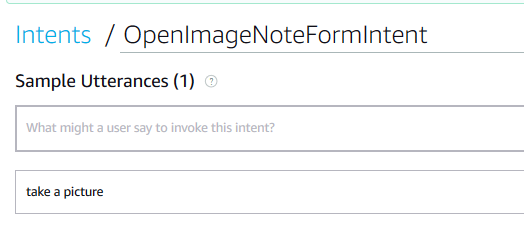
\includegraphics[width=8cm]{intent_image}
\end{center}
\caption{OpenImageNoteFormIntent}
\label{OpenImageNoteFormIntent}
\end{figure}

\subsection{Izvajanje ''Skill-a'' po korakih}

Alexa ''Skill'' se bo začel izvajati, ko uporabnik izreče definirano invokacijsko frazo.
Alexa posnet govorni ukaz pošlje na Amazonov Alexa Server.
Tam se s pomočjo NLU razpoznavnega modela poskusi pretvoriti v znakovni niz.
Ta znakovni niz se primerja z vsemi definiranimi invokacijskimi frazami za ''Skill-e'', ki so vezani na naš Amazon račun.

Če Alexa Server uporabnikov glasovni ukaz razpozna kot ,,make a report note'', se začne izvajati OpenReportAlexaSkill.
V ozadno kodo ''Skill-a'' (ang. Endpoint) se pošlje zahteva tipa \texttt{LaunchRequest}.

''Endpoint'' nastavimo v Alexa Developer nadzorni plošči (Slika \ref{skill_endpoint}).
To je lahko AWS Lambda funkcija, lahko pa je naš lasten strežnik, dostopen preko javne domene.
''Endpoint'' je v našem primeru gostovan na storitvi AWS Lambda.
Ob prejetju \texttt{LaunchRequest} ''Endpoint'' našega ''Skill-a'' vrne vprašanje ''What now?''.

\begin{figure}[H]
\begin{center}
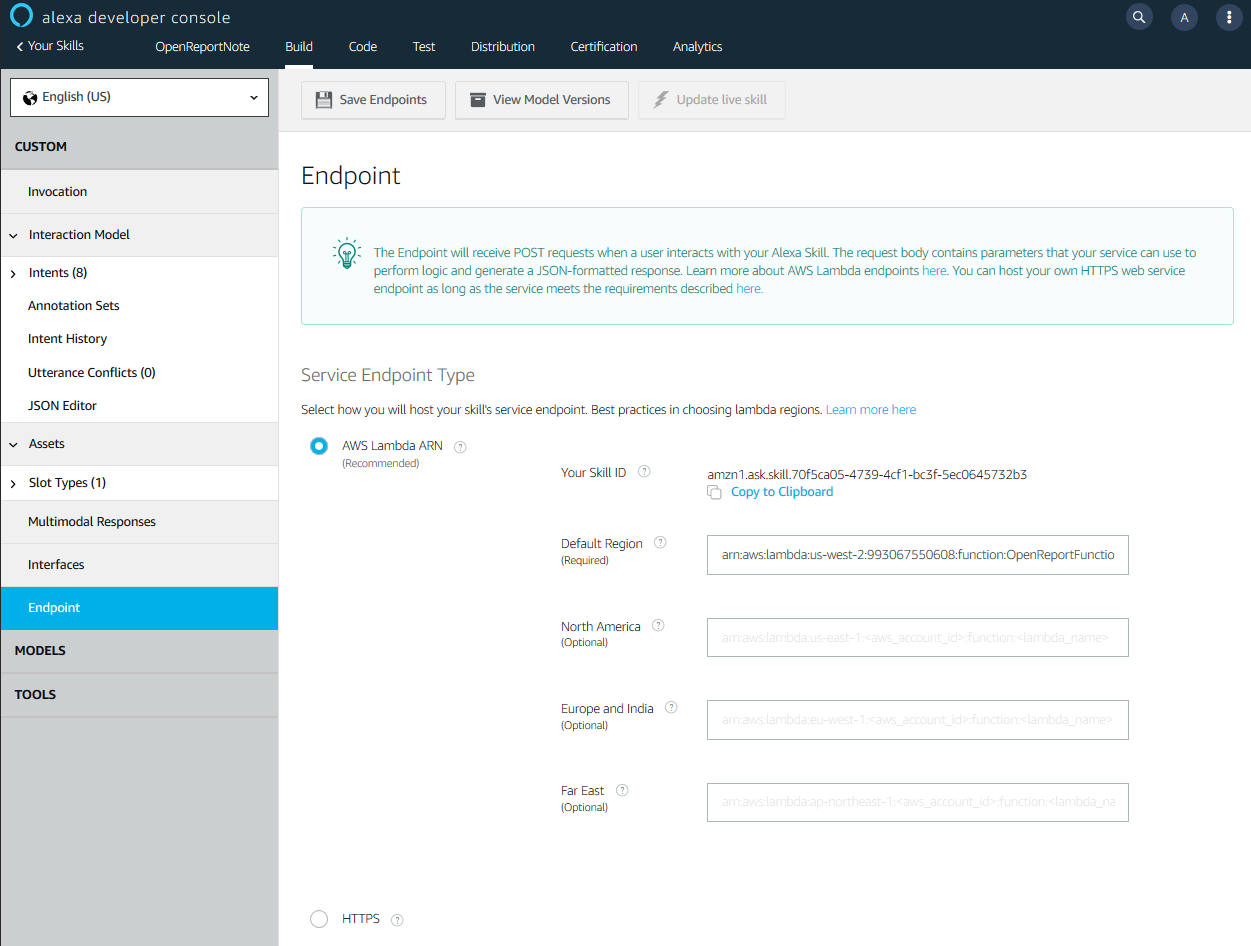
\includegraphics[width=13cm]{skill_endpoint}
\end{center}
\caption{''Endpoint'' OpenReportAlexaSkill-a v Alexa Developer nadzorni plošči}
\label{skill_endpoint}
\end{figure}

Naslednji glasovni ukaz se primerja s frazami za namere (ang. Intent).
Če se ukaz ujema z frazami, ki zaženejo katerega od ''Intent-ov'' TakeNoteIntent, OpenTextNoteFormIntent ali OpenImageNoteFormIntent, se na ''Endpoint'' pošlje zahteva tipa \texttt{IntentRequest}.

Iz prejetega \texttt{IntentRequest}-a nato dobimo ime ''Intent-a''.
Na podlagi imena prejetega Intent-a ločimo, ali gre za TakeNoteIntent, OpenTextNoteFormIntent ali OpenImageNoteFormIntent in zaženemo funkcije, opisane v prejšnjem poglavju.

Oris obdelave invokacije ''Skill-a'' in namere \texttt{TakeNoteIntent} je prikazan s spodnjo sliko (slika \ref{skill}).
\begin{figure}[H]
\begin{center}
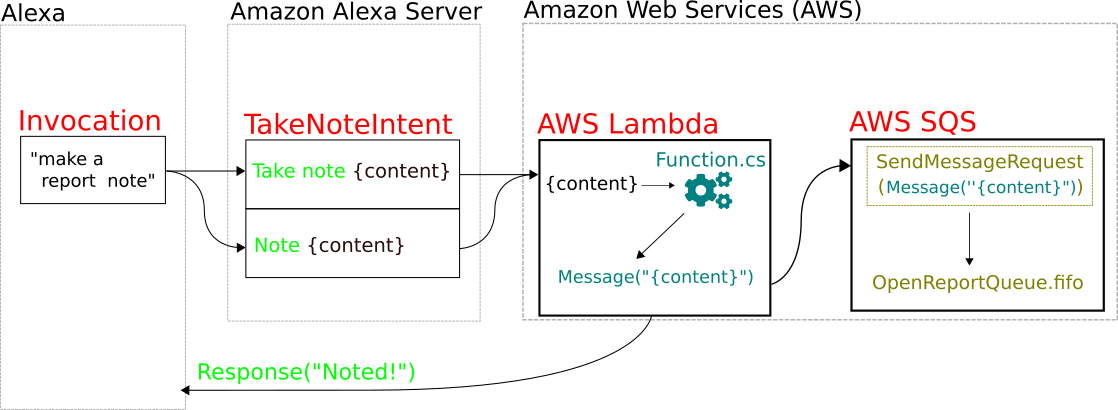
\includegraphics[width=13.5cm]{skill_2}
\end{center}
\caption{Načrt Alexa Skilla}
\label{skill}
\end{figure}

\subsection{Ovire pri izdelavi Alexa ''Skill-a''}

Pri implementaciji Alexa ''Skill-a'' smo naleteli na najbolj očitne težave v sklopu te raziskave.

Prva je bila jezikovne narave, saj Alexa ne podpira prepoznavanja slovenskega jezika.

Naslednja težava je bila izbira prave invokacijske fraze.
Fraze, kot so ''take a note'' ali ''take a picture'' so že rezervirane v sklopu Alexinih privzetih funkcionalnosti.
Težavo je predstavljalo izbrati frazo, je bila hkrati kratka, intuitivna in se ni napačno interpretirala v invokacijsko frazo privzetih funkcionalnosti.
Invokacija ''make a report note'' je bila najboljši kompromis, ki smo ga našli.

Težavo je predstavljalo tudi razpoznavanje dolgih stavkov, še posebej, če se ti niso ujemali z definiranimi frazami namer.
To je zelo omejilo možnost narekovanja besedila korakov s pomočjo Amazon Alexe.

Naslednjo težavo je predstavljal čas, ki ga je Alexa porabila za interpretacijo definiranih glasovnih ukazov.
Za procesiranje glasovnih ukazov je porabila v povprečju od 3 do 6 sekund.

\section{Implementacija mobilne aplikacije}

Mobilno aplikacijo bomo uporabili kot primer klienta za naš strežnik.

Do strežnika bo dostopala preko API vmesnika.
Zahtevki se bodo prenašali preko HTTP protokola.

Mobilno aplikacijo smo se odločili razviti s tehnologijo Xamarin.
Razlogi za to so predvsem dobro poznavanje tehnologije in enostavna integracija z ostalimi tehnologijami iz .NET sklopa.


\subsection{Pristop}
Pristop razvoja aplikacije, ki smo ga uporabili za programiranje aplikacije, se imenuje ''Model View View-Model'' (v nadaljevanju MVVM).
Pri tem pristopu aplikacijo razdelimo na tri dele (Slika \ref{mvvm}).

\textbf{Model} je del, kjer definiramo elemente naše ''poslovne logike'' (opis tehnološkega postopka, korak, uporabnik,...).

\textbf{View} je uporabniški vmesnik, ki ga vidi uporabnik.

\textbf{ViewModel} pa se uporablja, da se poveže funkcije uporabniškega vmesnika in modela (''poslovne logike'') ter po potrebi preoblikuje podatke.

Rezultat upoštevanja tega pristopa je čista koda, ki nima prepletenih elementov med ozadno kodo in uporabniškim vmesnikom.
''Model'' vsebuje le abstrakcijo naših podatkov in ''poslovno logiko''.
Ti podatki se v ''ViewModel-u'' pretvorijo v obliko, ki bo prikazana uporabniku.
''View'' pa nato servira pripravljene podatke uporabniku v obliki grafičnih elementov.

\begin{figure}[H]
\begin{center}
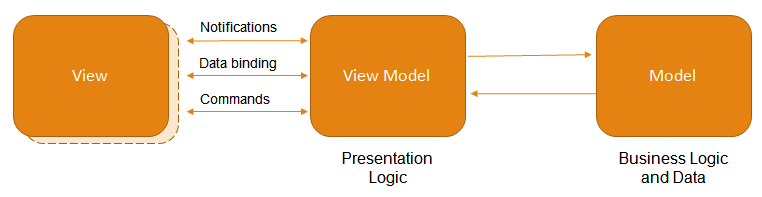
\includegraphics[width=11cm]{mvvm}
\end{center}
	\caption{Shema pristopa MVVM}
\label{mvvm}
\end{figure}

\subsection{Povezava na strežnik, prijava in registracija uporabnika}

Za kreiranje in avtorizacijo HTTP zahtevkov v okviru aplikacije skrbi storitev za komunikacijo s strežnikom (razred \\\texttt{OpenReportServerCommunicationService.cs}).
Storitev se registrira ob zagonu aplikacije po metodi Dependency Injection.
Za to metodo registracije storitev smo se odločili, saj omogoča enostavno uporabo instanc registriranih storitev kjerkoli v aplikaciji.

Ob zagonu mobilne aplikacije, uporabnika pričaka stran za povezavo na OpenReport strežnik.
V tekstovno polje mora vpisati URL ali IP naslov strežnika.
Ta naslov bomo v nadaljevanju podpoglavja označevali z \texttt{naslovstrežnika}.

% // slika povezavne strani

\begin{figure}[H]
\begin{center}
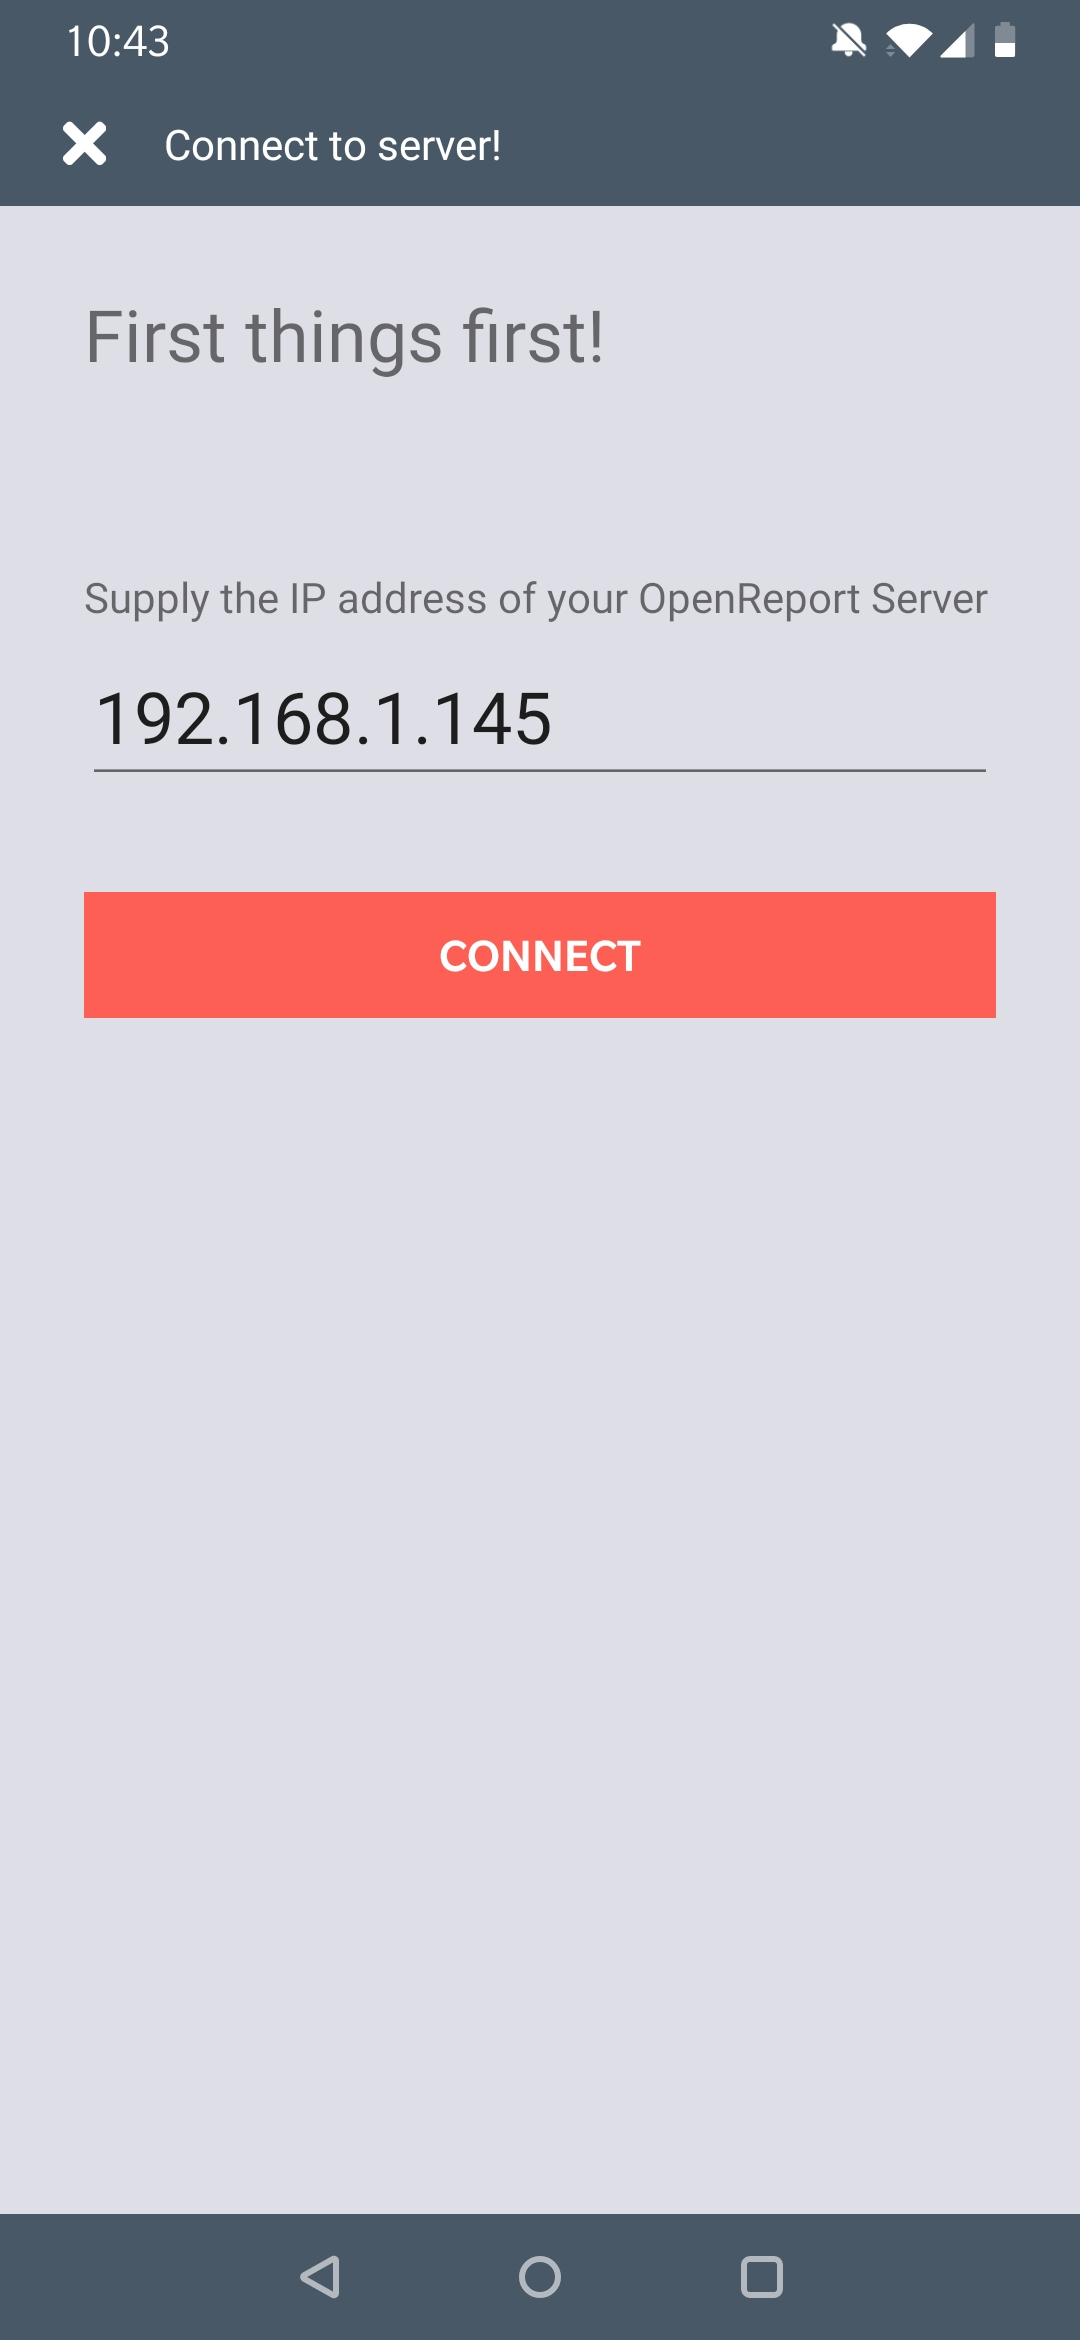
\includegraphics[width=4cm]{app_connect}
\end{center}
\caption{Povezavna stran}
\label{app_connect}
\end{figure}

Ko uporabnik pritisne na gumb ''Connect'', se preveri, ali je naslov pravilno formuliran.
Če je, storitev za komunikacijo s strežnikom pošlje neavtorizirano GET zahtevo na ''\texttt{naslovstrežnika}/connect''. 
Če je na tem naslovu res OpenReport strežnik, se kot odgovor odjemalcu pošlje boolean vrednost \texttt{true}.

Storitev za komunikacijo s strežnikom si nato hrani vrednost \texttt{naslovstrežnika} kot predpono vseh nadaljnjih zahtevkov.

Ob neuspešnem poskusu povezave se uporabniku na strani prikaže opis napake.
Če je poskus uspešen, se stran za povezavo na strežnik zapre.

Prikaže se stran za prijavo.
Na tej strani uporabnik vpiše svoje uporabniško ime ali geslo, lahko pa odpre stran za registracijo računa.


\begin{figure}[H]
\begin{center}
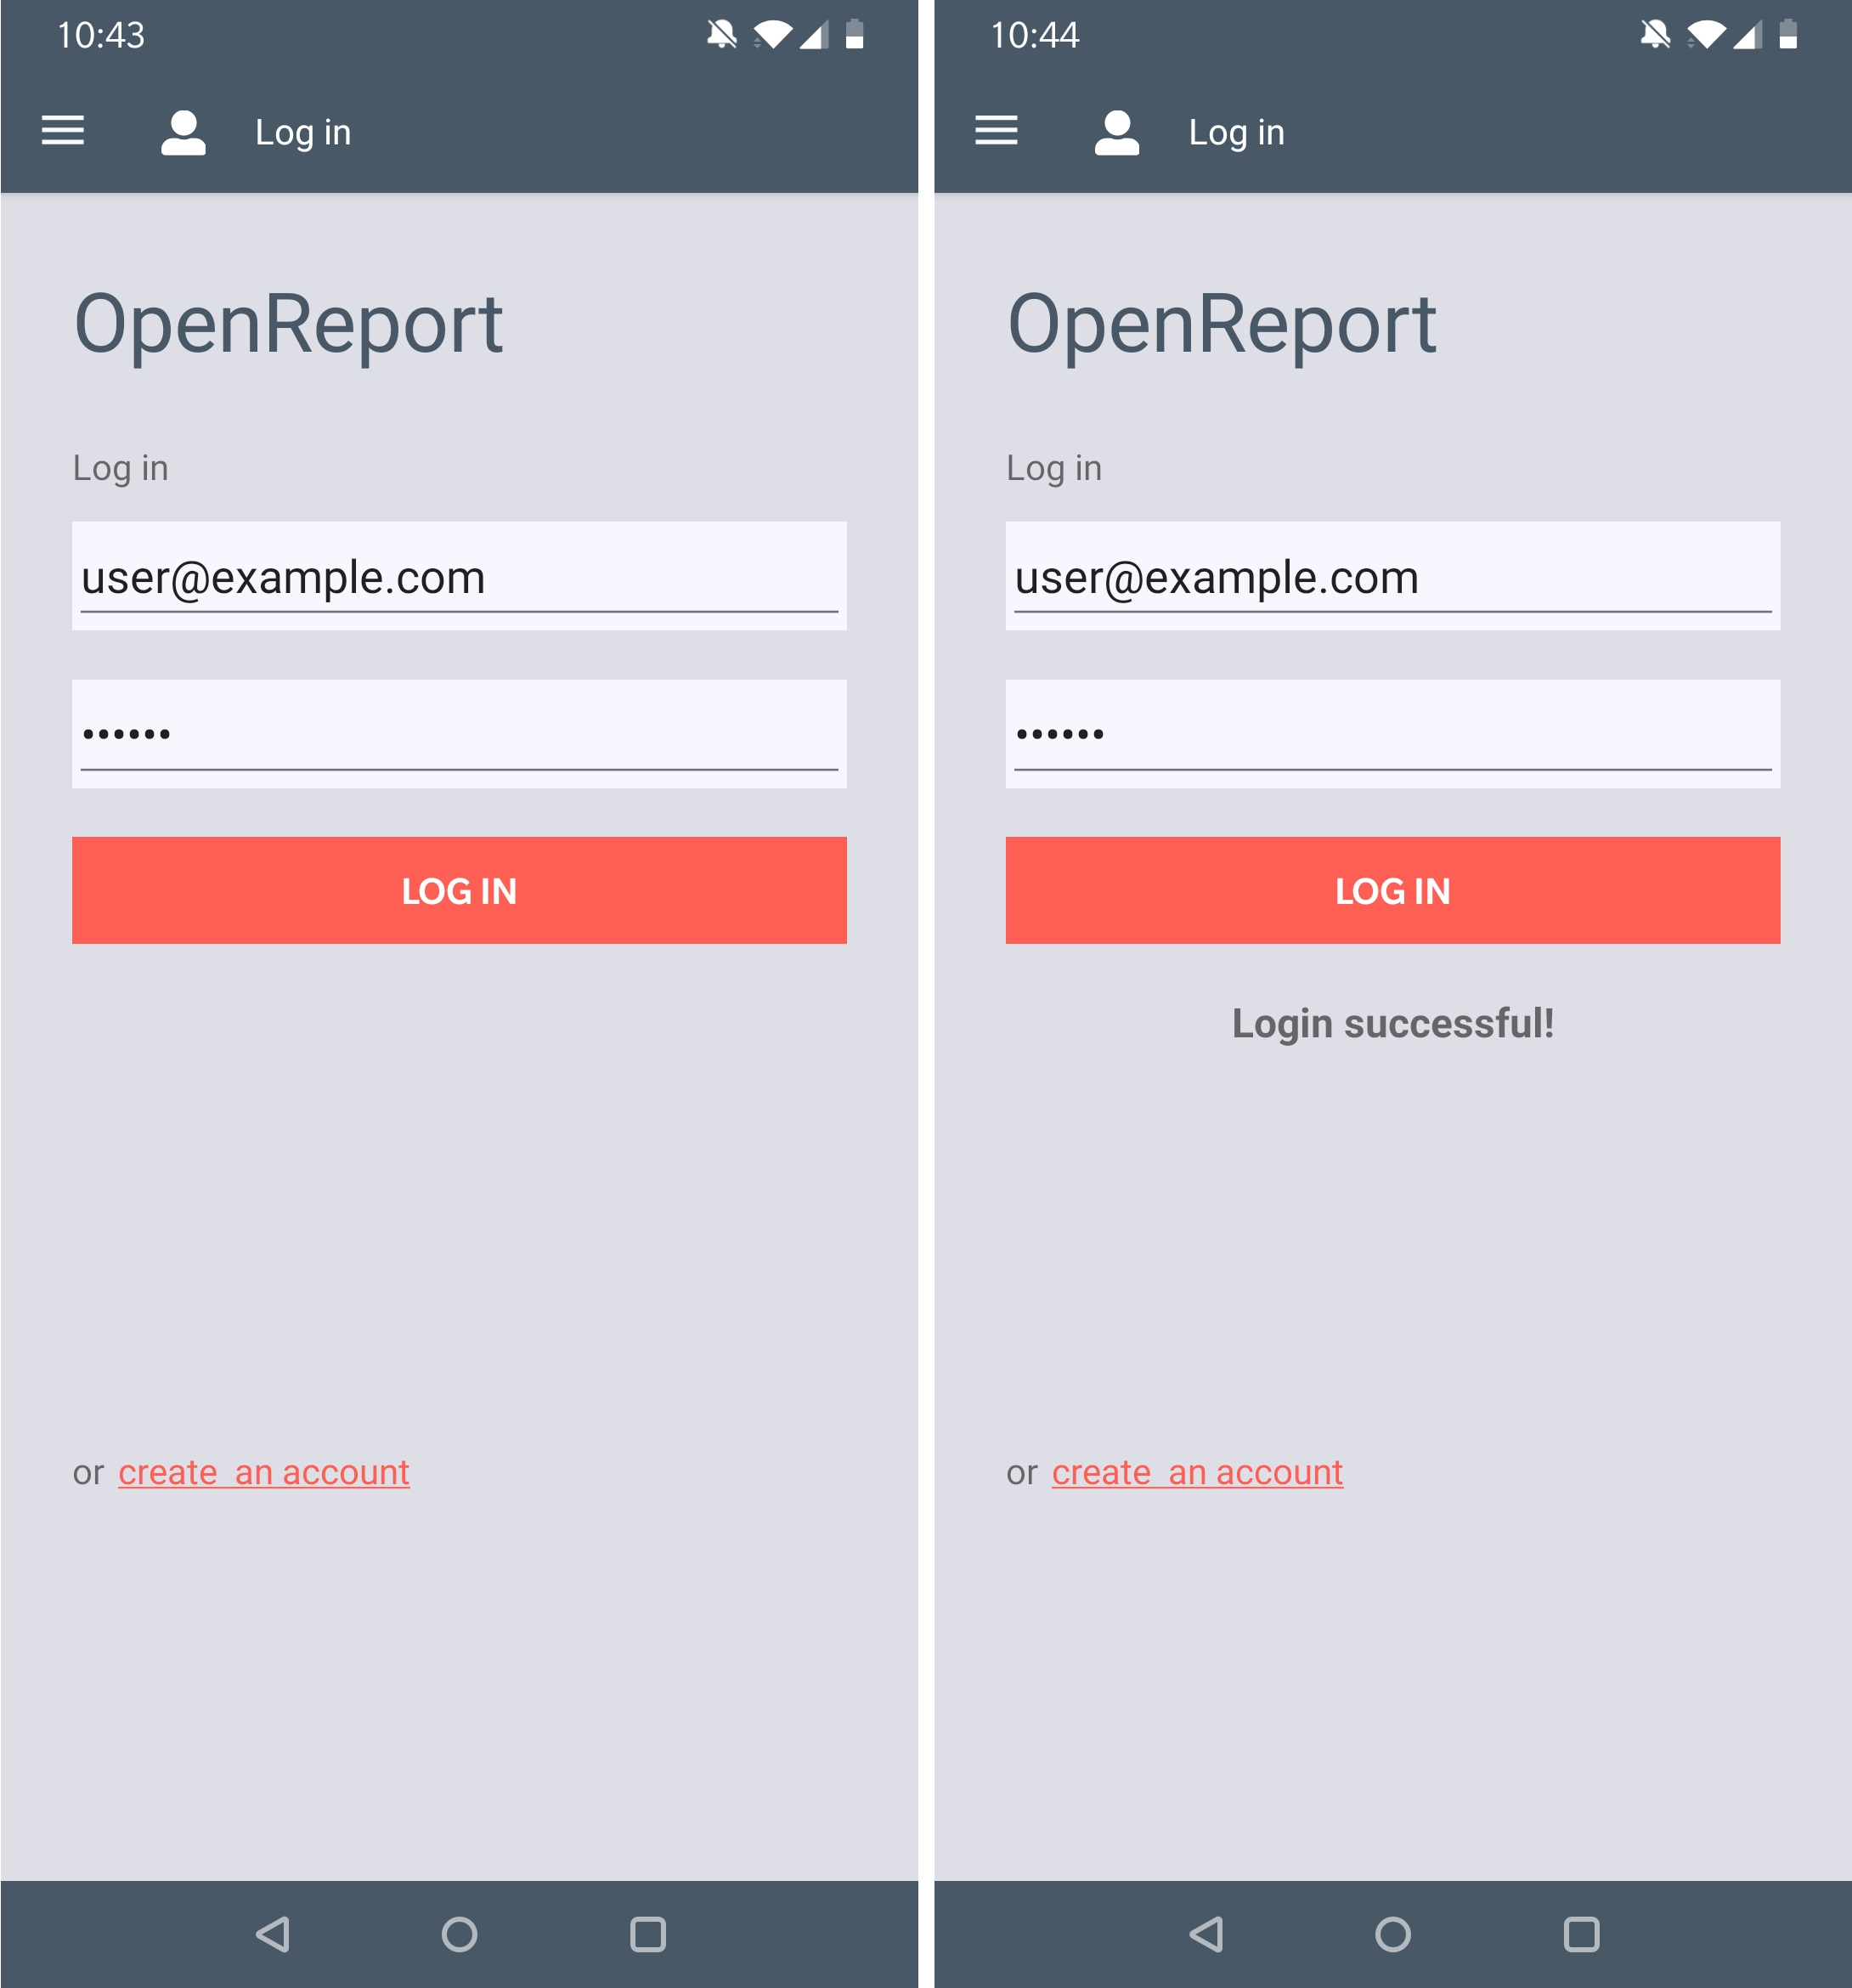
\includegraphics[width=8cm]{app_login}
\end{center}
	\caption{Prijavna stran pred poskusom prijave (levo), in po uspešnem poskusu prijave (desno)}
\label{app_login}
\end{figure}


Za prijavo in registracijo skrbi avtentikacijska storitev (razred \\\texttt{IdentityService.cs}).
Ta storitev je enako kot storitev za komunikacijo registrirana z Dependency Injection.
Pogoj, da jo lahko koristimo, je, da je storitev za komunikacijo uspešno vzpostavila komunikacijo s strežnikom.

Poskus prijave poteka tako, avtentikacijska storitev uporabniško ime in geslo iz prijavne strani zapiše v objekt razreda \texttt{LoginUserRequest}.

\begin{Verbatim}[commandchars=+\[\]]
LoginUserRequest {
    string Email; 
    string Password;
}
\end{Verbatim}

Nato se ta objekt pošlje na strežnik na URL ''\texttt{/identity/login}'' preko POST metode.
Strežnik ob uspešni avtentikaciji vrne objekt razreda \texttt{AuthSuccessResponse}.
Iz tega objekta uporabnik prebere svoj avtorizacijski žeton.
Ta žeton hrani avtentikacijska storitev.
Pri nadaljnjih poizvedbah komunikacijska storitev ta žeton doda v glavo HTTP zahtevkov.

Če je avtentikacija neuspešna, strežnik vrne objekt razreda \texttt{AuthFailedResponse}, v katerem je podan opis napake.
Ta opis napake se nato uporabniku izpiše na prijavni strani.

Stran za registracijo (slika \ref{app_register}) je podobna strani za prijavo, le da ima dve vnosni polji za vpis gesla.
Drugo vnosno polje je preventivni ukrep, da se uporabnik ne registrira z napačno vtipkanim geslom.

Registracijski zahtevek se pošlje na strežnik na URL ''\texttt{/identity/register}''.
Zahtevek je objekt razreda \texttt{RegisterUserRequest}.

\begin{Verbatim}[commandchars=+\[\]]
RegisterUserRequest {
    string Email; 
    string Password;
}
\end{Verbatim}

\begin{figure}[H]
\begin{center}
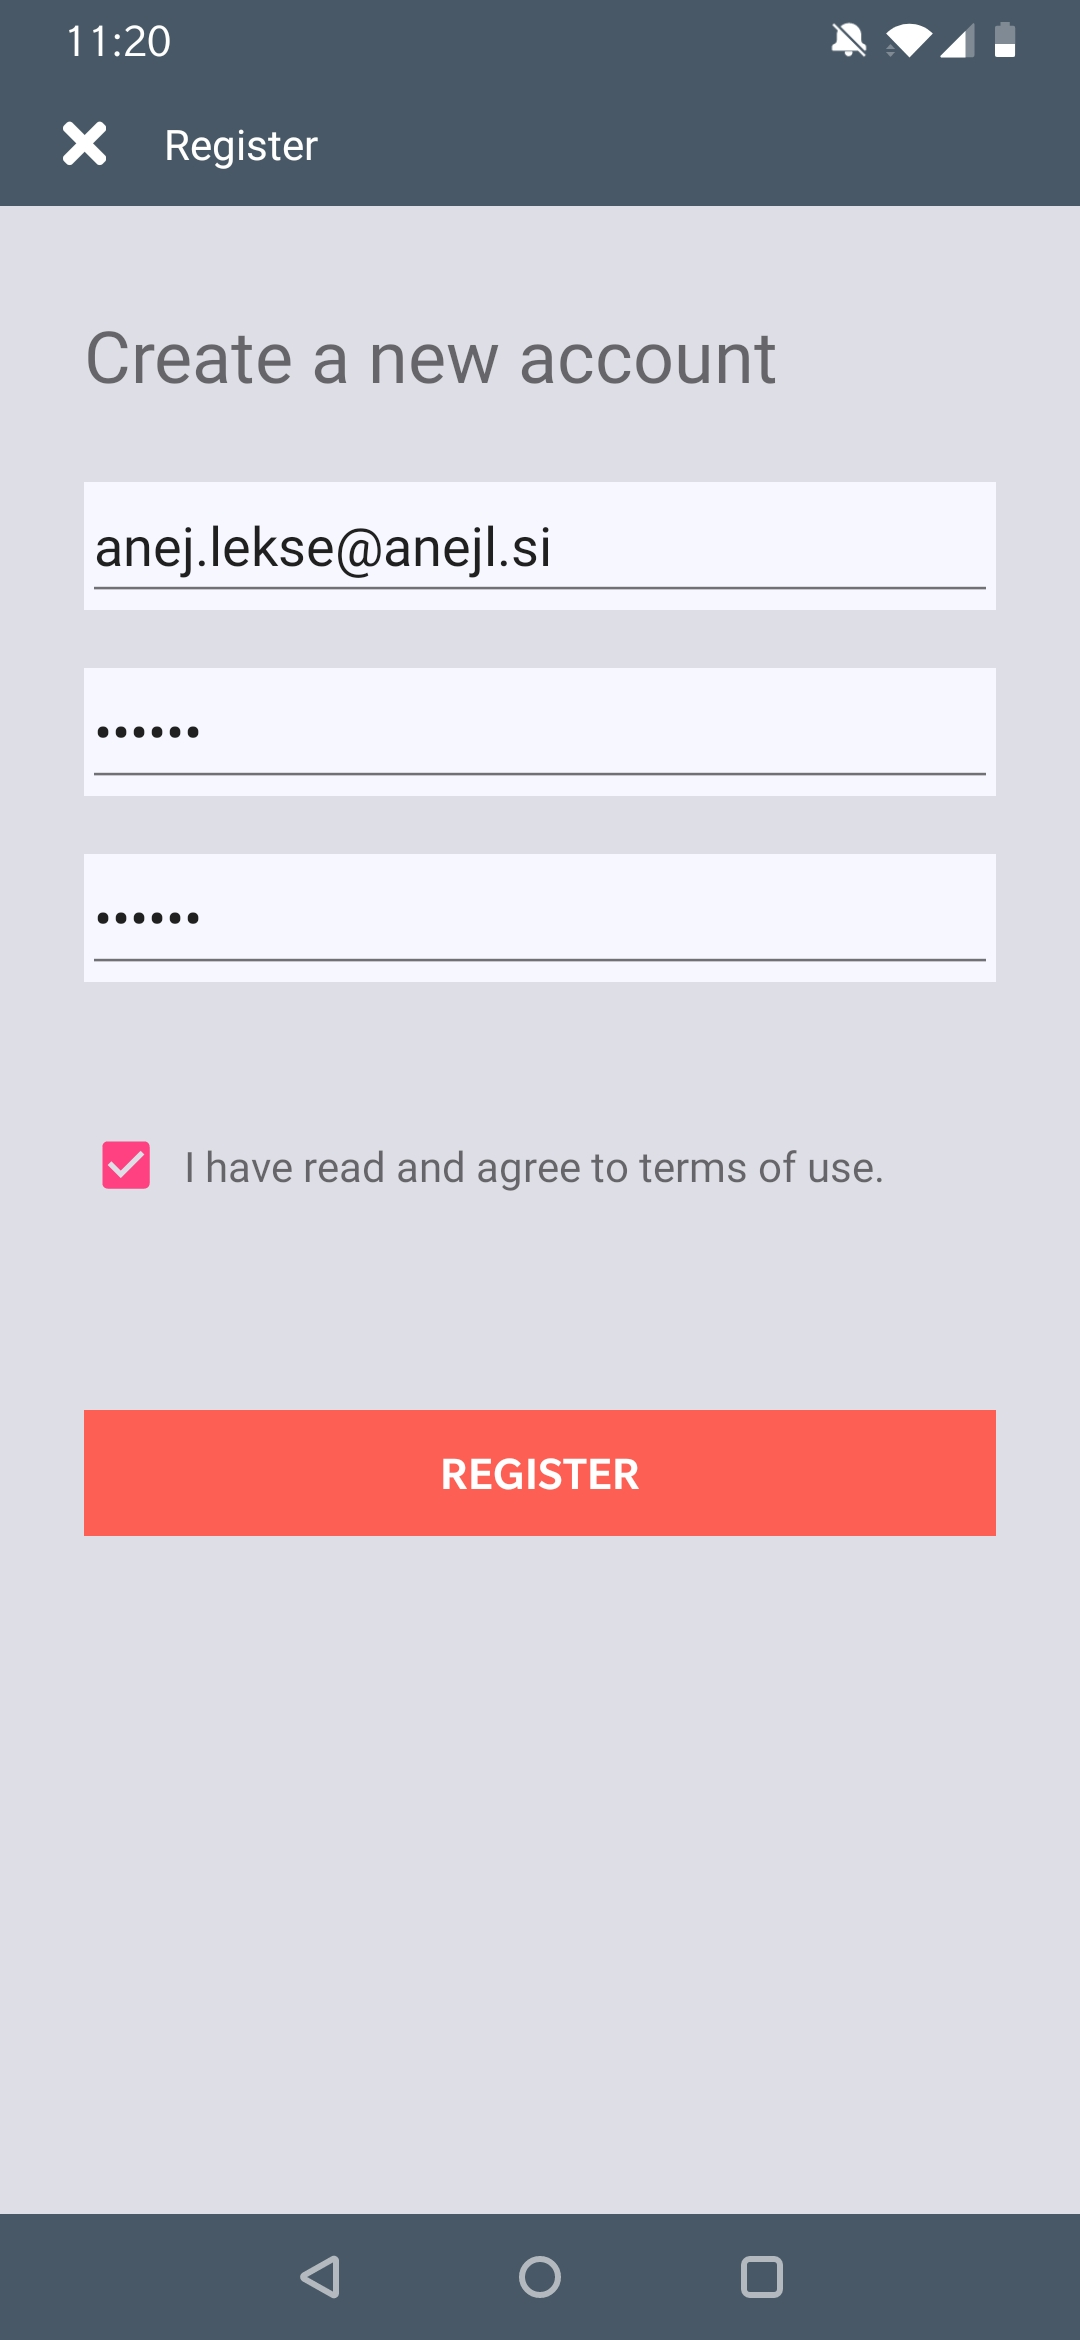
\includegraphics[width=4cm]{app_register}
\end{center}
	\caption{Registracijska stran}
\label{app_register}
\end{figure}

\subsection{Ustvarjanje, brisanje in odpiranje projektov}

Po prijavi lahko uporabnik odpre stran s projekti.
Na tej strani se prikažejo:
\begin{itemize}
	\item seznam vseh njegovih projektov, 
	\item gumbi za izbris posameznega projekta,
	\item gumb za dodajanje novega projekta in
	\item gumb za zahtevanje in izpust glasovnega asistenta.
\end{itemize}

\subsubsection{Ustvarjanje novega projekta}

Za ustvarjanje novega projekta (slika \ref{app_newproject}), mora na strani za ustvarjanje projektov uporabnik vpisati naslov projekta (\texttt{Title}), kratek opis (\texttt{Description} in našteti možne nevarnosti pri delu \texttt{Dangers}.

Te tri vrednosti se zapišejo v objekt razreda \texttt{CreateProjectRequest}.
\begin{Verbatim}[commandchars=+\[\]]
CreateProjectRequest {
    string Title;
    string Description;
    string Dangers;
}
\end{Verbatim}

Ta objekt nato storitev za komunikacijo s strežnikom pošlje preko metode POST na URL ''\texttt{/projects/create}''.
Strežnik v odgovor vrne objekt razreda \texttt{Project}, ki ga je zahtevek ustvaril.

Nov projekt se nato prikaže v seznamu vseh uporabnikovih projektov na strani ''Dashboard'', kjer ga lahko uporabnik odpre ali izbriše.

\begin{figure}[H]
\begin{center}
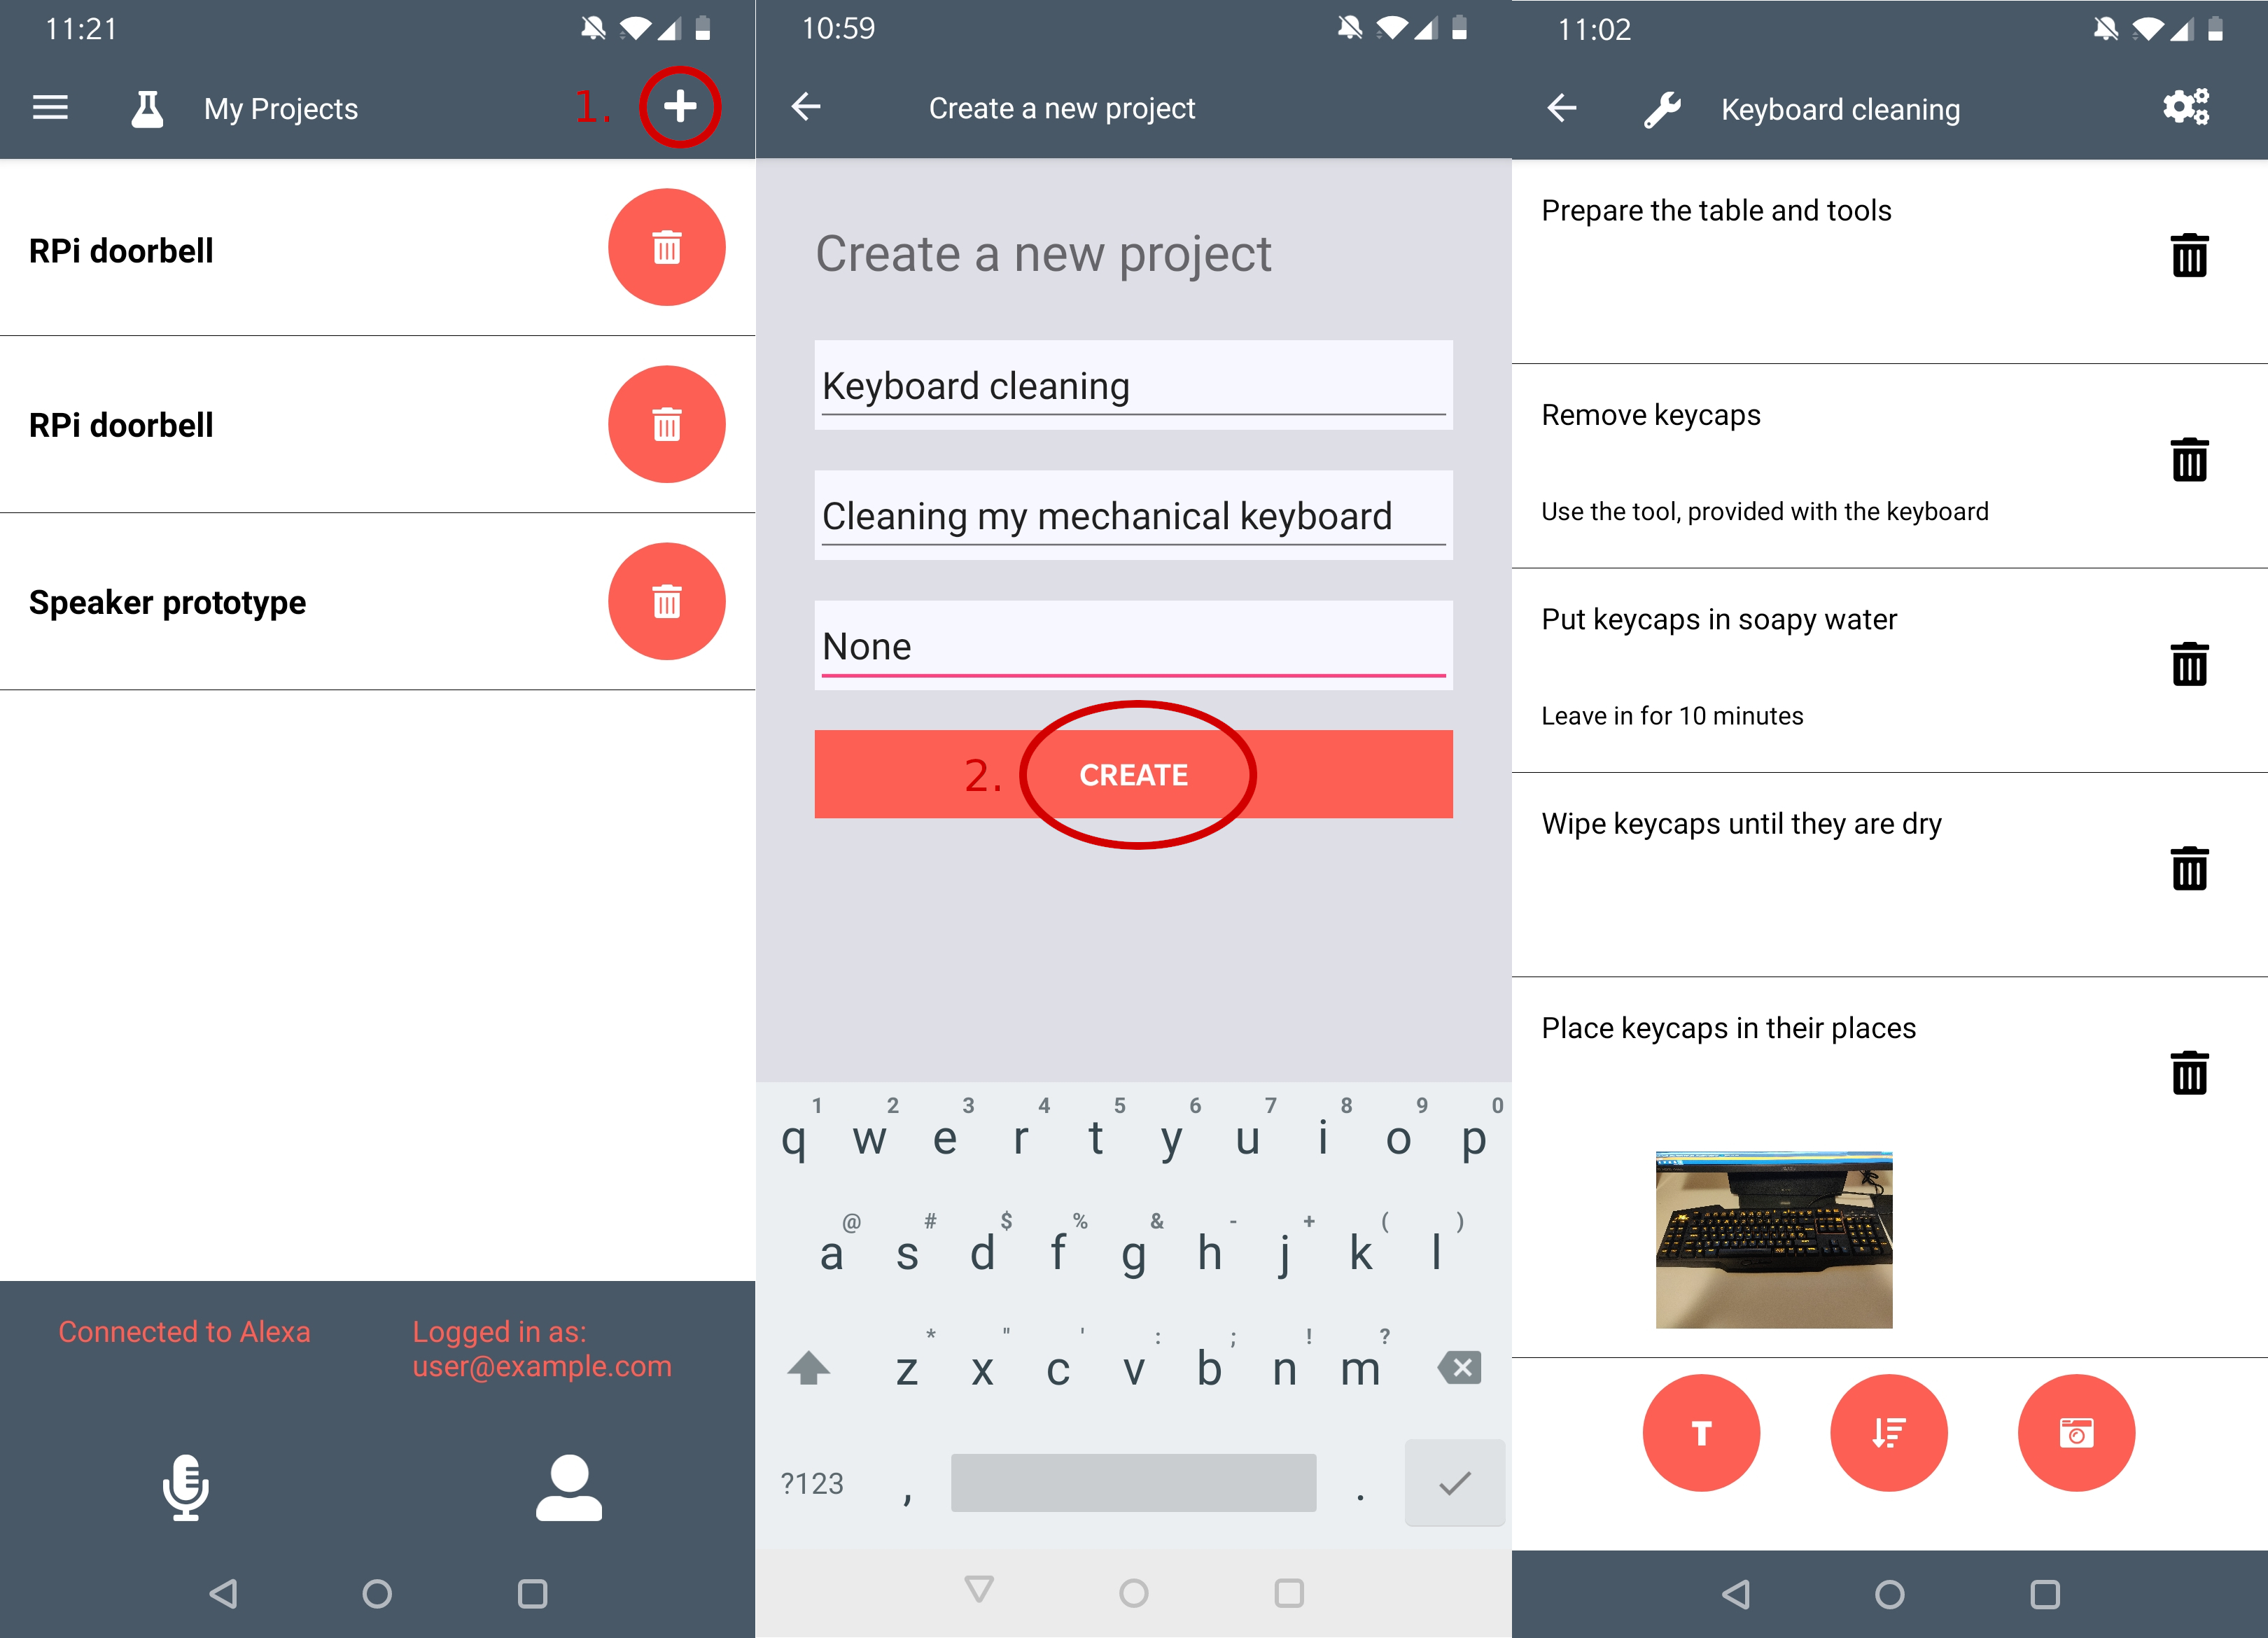
\includegraphics[width=13cm]{app_newproject}
\end{center}
	\caption{Postopek ustvarjanja novega projekta po korakih.}
\label{app_newproject}
\end{figure}

\subsubsection{Izbris projekta}

Da uporabnik izbriše projekt, mora na strani ''Dashboard'' ob željenem projektu tapniti na gumb z ikono smetnjaka.
Pritisk na ta gumb sporoči storitvi za komunikacijo s strežnikom, naj pošlje avtoriziran DELETE zahtevek na URL ''\texttt{/projects/\{id\}/delete}''.
Strežnik ob uspešnem izbrisu projekta odjemalcu vrne kopijo izbrisanega projekta.

\subsection{Zahtevanje in izpust glasovnega asistenta}

Za zahtevanje in izpust glasovnega asistenta v mobilni aplikaciji skrbi storitev za upravljanje z glasovnim asistentom (razred \texttt{VoiceAssistantService.cs}).
Ta se registrira ob začetku izvajanja aplikacije, nato pa počaka, da avtentikacijska storitev uspešno opravi prijavo uporabnika.
Takrat storitev na URL ''\texttt{/users/current}'' pošlje zahtevek GET.

Strežnik vrne \texttt{User} objekt trenutnega uporabnika.
Iz tega objekta storitev za upravljanje z glasovnim asistentom preveri, ali ima nase vezanega glasovnega asistenta, tako da preveri vrednost boolean polja \texttt{UsesVoiceAssistant}.

Če ima uporabnik vrednost polja \texttt{UsesVoiceAssistant} nastavljeno na \texttt{true}, lahko uporablja glasovnega asistenta.

Če ima uporabnik vrednost polja \texttt{UsesVoiceAssistant} nastavljeno na \texttt{false}, mora uporabo glasovnega asistenta zahtevati.
To naredi tako, da pošlje avtoriziran PUT zahtevek (brez vsebine) na URL ''\texttt{/users/requestva}''.

Če noben drug prijavljen uporabnik nima polja \texttt{UsesVoiceAssistant} nastavljenega na \texttt{true}, se njegova zahteva odobri.
V njegovem objektu \texttt{User} se nastavi vrednost \texttt{UsesVoiceAssistant} na \texttt{true}.
Če pa ima kateri od uporabnikov to polje nastavljeno na \texttt{true}, pa mora počakati, da uporabnik, ki asistenta uporablja, asistenta izpusti.
Ko si asistenta ne lasti nobeden drug uporabnik, ga lahko veže nase.

Izpust asistenta dosežemo, da uporabnik, ki asistenta trentuno uporablja, pošlje avtoriziran PUT zahtevek na URL ''\texttt{/users/releaseva}''.

V mobilni aplikaciji zahtevanje in izpust asistenta nadziramo na ''Dashboard'' strani, s pritiskom na ikono mikrofona.

\begin{figure}[H]
\begin{center}
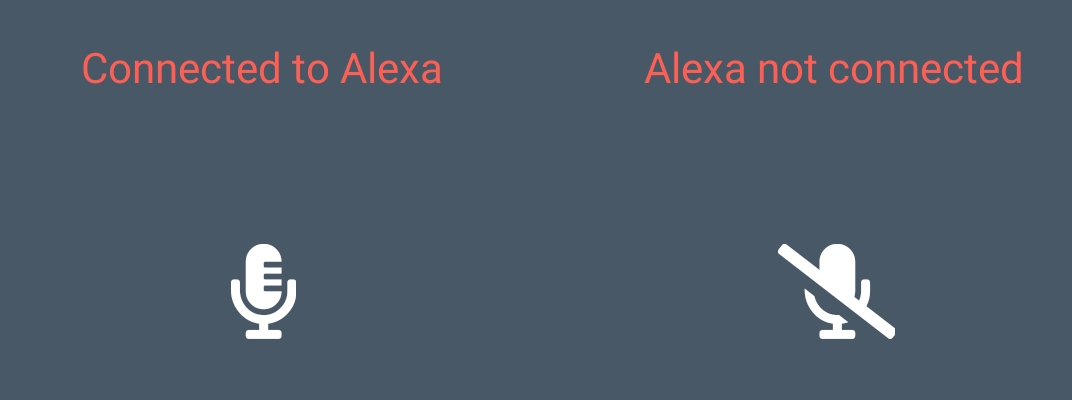
\includegraphics[width=7cm]{app_alexa_yesno}
\end{center}
	\caption{Gumb v obeh stanjih}
\label{app_alexa_yesno}
\end{figure}

\subsection{Odpiranje in sinhronizacija projekta}

Ko uporabnik iz seznama izbere projekt, ki ga želi odpreti, storitev za komunikacijo s strežnikom pošlje na URL ''\texttt{/projects/\{id\}/notes}'' zahtevek GET.
Polje \texttt{\{id\}} je v tem primeru unikatni identifikator željenega projekta.

Storitev za projekte (razred \texttt{ProjectService.cs}) nato prejet odgovor, razreda \texttt{Project}, hrani.
Vse korake, ki pripadajo temu projektu, se hrani v seznam tipa ObservableCollection.
Seznam nato prikažemo na strani za upravljanje s projektom.
Ta tip seznama smo izbrali, saj je nad njim najlažje opravljati zamenjevalne operacije.

Storitev nato začne s periodično sinhronizacijo projekta.
To poteka tako, da storitev za projekte na URL ''\texttt{/projects/\{id\}/nonotes}'' pošlje avtoriziran GET zahtevek.
Strežnik v odgovor vrne objekt razreda \texttt{Project} s praznim seznamom korakov.
Vse, kar gledamo, je vrednost zastavic \texttt{NoteRequest}, \texttt{ImageRequest} in \texttt{AlexaNoteRequest}.

Če ima novo prejeti projekt nastavljeno zastavico \texttt{NoteRequest}, storitev odpre obrazec za dodajanje novega tekstovnega koraka v projekt.

Če ima novo prejeti projekt nastavljeno zastavico \texttt{ImageRequest}, storitev za projekte odpre obrazec za dodajanje nove fotografije.

Če ima novo prejeti projekt nastavljeno zastavico \texttt{AlexaNoteRequest}, storitev za projekte pošlje avtoriziran GET zahtevek na URL ''\texttt{/projects/\{id\}/notes}''.
Polje \{id\} mora v tem primeru biti unikatni identifikator odprtega projekta.
V odgovor prejme objekt razreda \texttt{Project}, vključno s seznamom vseh korakov, ki mu pripadajo.
V prejetem seznamu je namreč tudi narekovan korak.
Storitev za projekte primerja, katerega od korakov še nima v svoji zbirki.
Ko ta korak najde ga doda v svoj ObservableCollection.

Ko se projekt sinhronizira, storitev za projekte pošlje na strežnik avtorizirano PUT zahtevo na URL ''\texttt{/project/last/closerequests}''.
Ta zahteva nastavi vrednost zastavic \texttt{NoteRequest}, \texttt{ImageRequest} in \texttt{AlexaNoteRequest} na \texttt{false}.


\subsection{Dodajanje in brisanje zapiskov}

Ko ima uporabnik projekt odprt, lahko vanj dodaja zapiske, jih briše, ureja in jim spreminja vrstni red.
Doda lahko tekstovni korak ali korak s fotografijo.

// TODO dodaj stran s fotografijami

\begin{figure}[H]
\begin{center}
	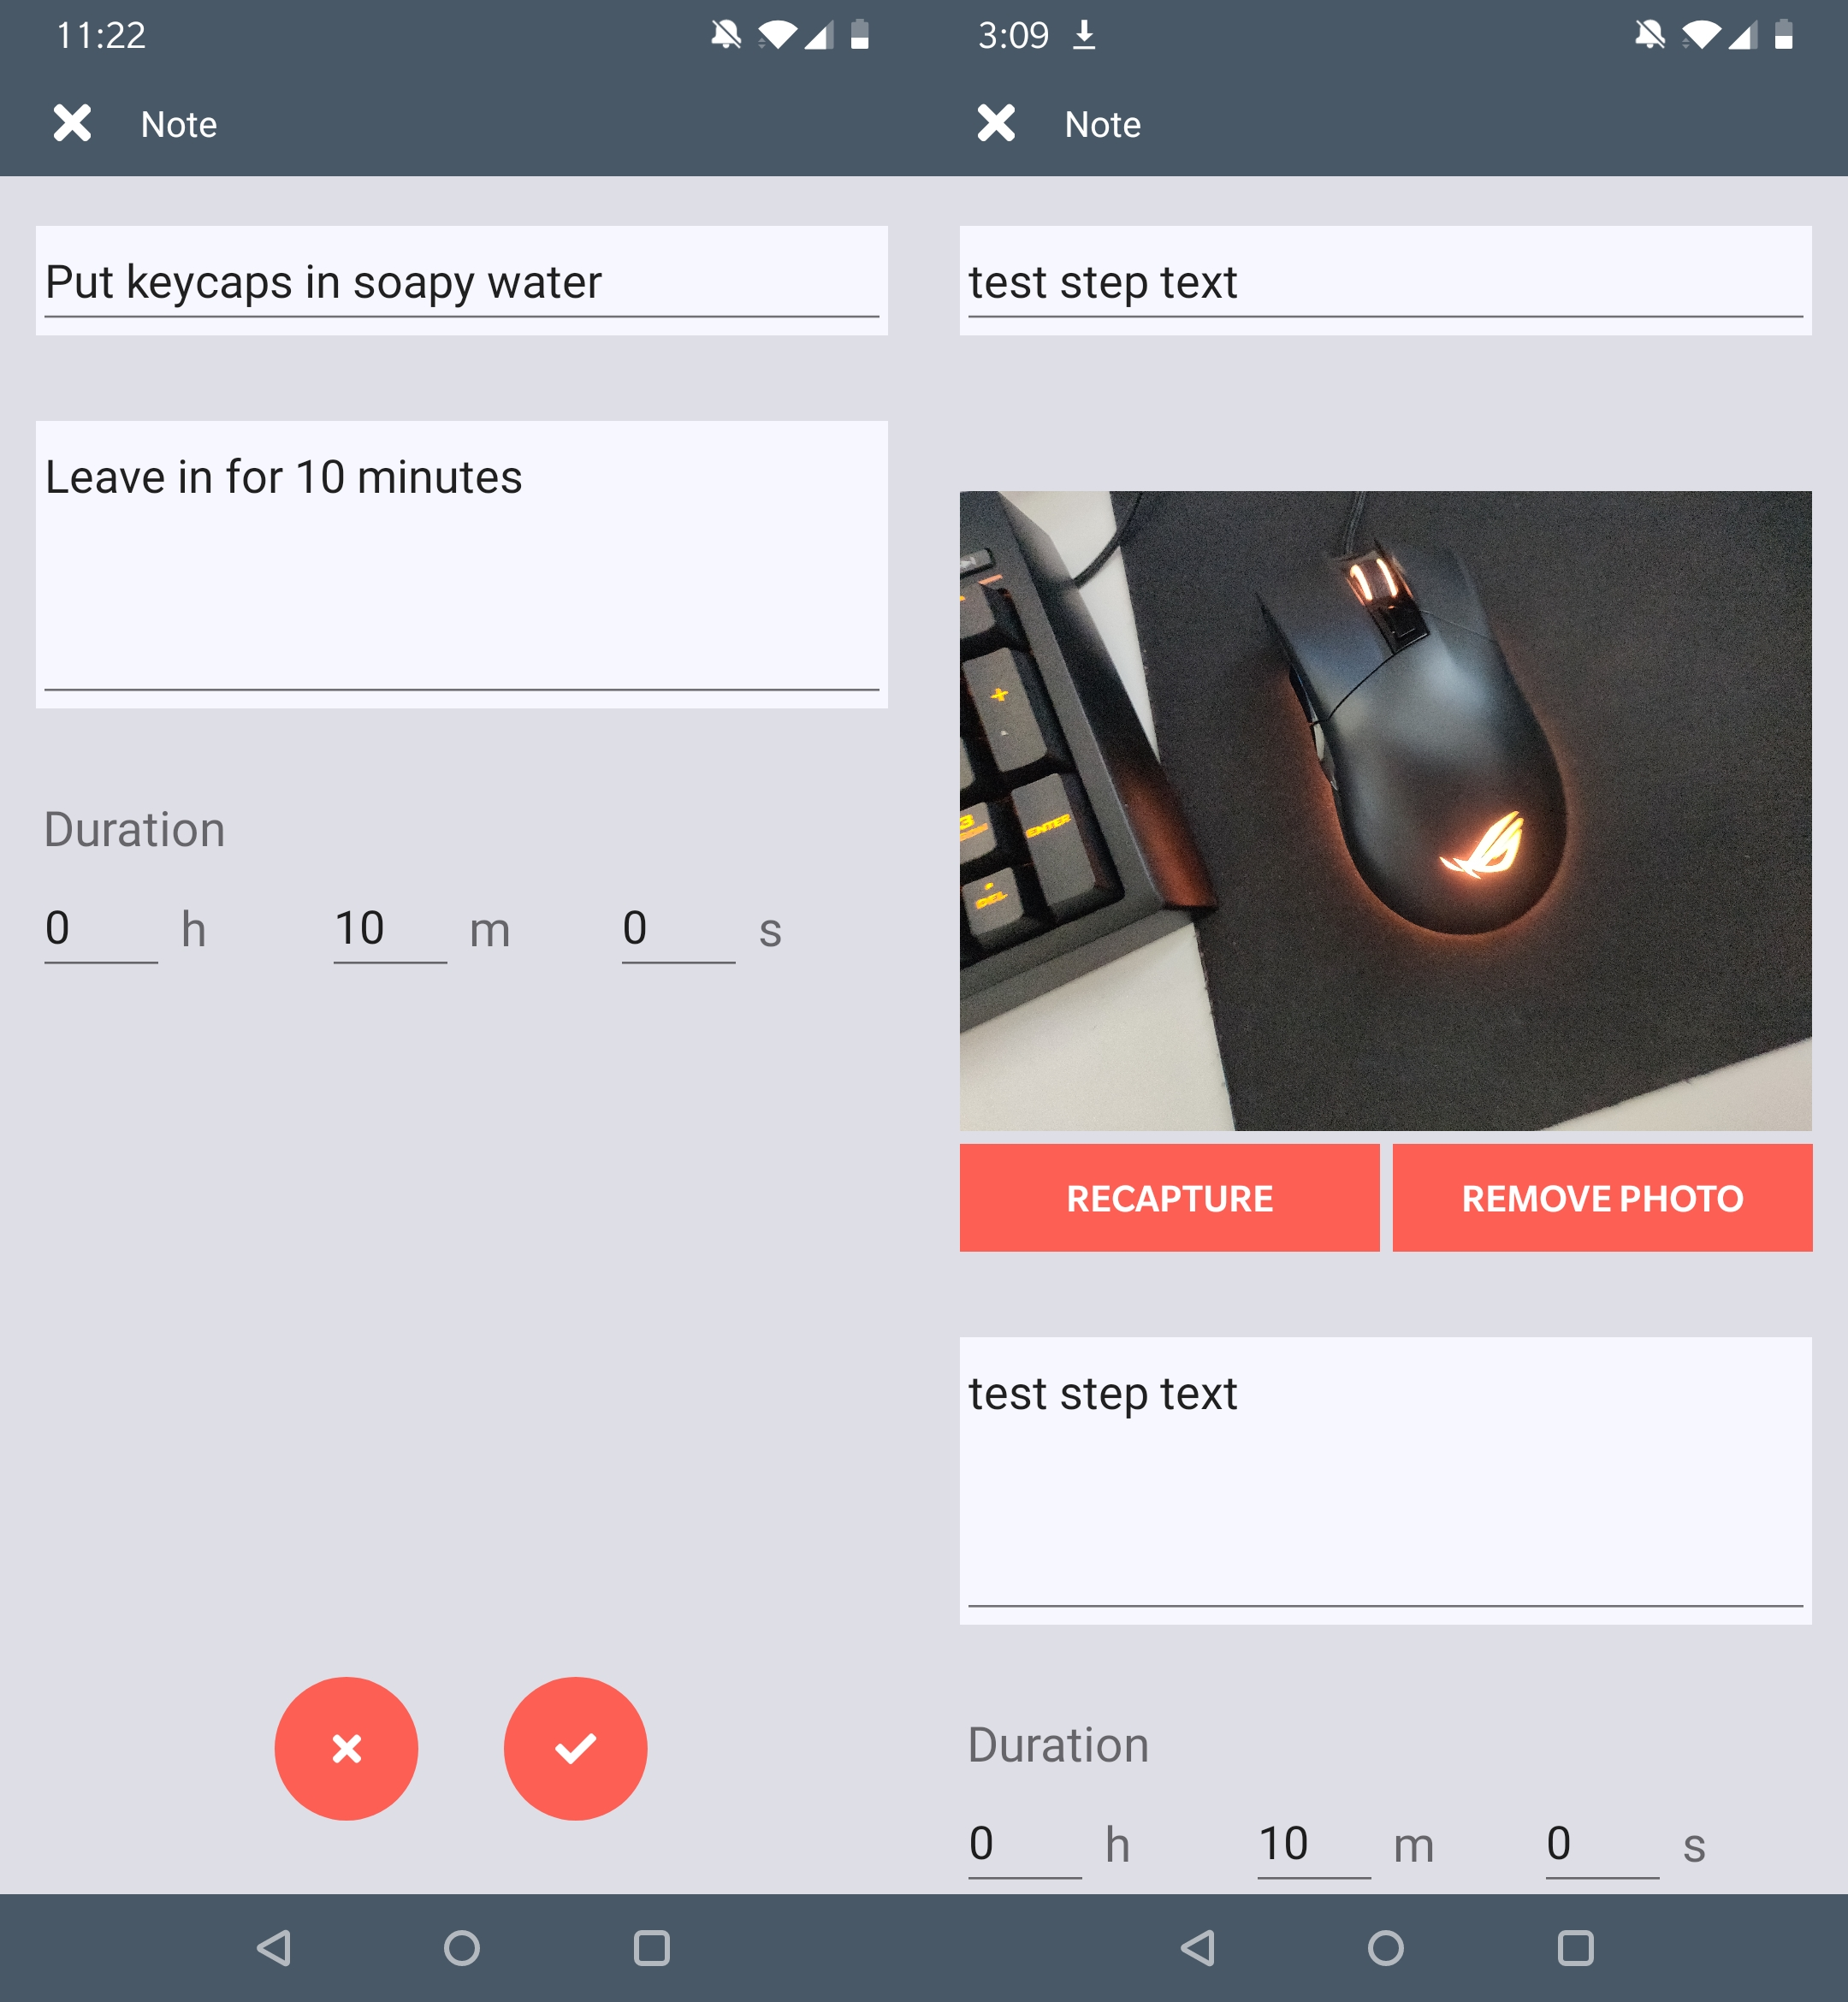
\includegraphics[width=4cm]{app_note_image}
\end{center}
	\caption{Stran za dodajanje/urejanje korakov}
\label{app_note}
\end{figure}

Pri dodajanju tekstovnega koraka mora uporabnik v vnosnem obrazcu podati naslov koraka (\texttt{Title}), opis koraka (\texttt{Text}) ter trajanje v urah, minutah in sekundah.
Ti podatki se nato hranijo v objektu razreda \texttt{Note}.
Ta objekt storitev za projekte zapakira v objekt tipa \texttt{AddNoteRequest} in ga pošlje storitvi za komunikacijo s strežnikom.

\begin{Verbatim}[commandchars=+\[\]]
AddNoteRequest { 
    Note note; 
}
\end{Verbatim}

Storitev za komunikacijo s strežnikom pošlje ta objekt na strežnik na naslov ''\texttt{/projects/\{id\}/addnote}''.
Polje \texttt{\{id\}} mora biti unikatni identifikator projekta, v katerega želimo korak vstaviti.
Če je vstavljanje v projekt uspešno, strežnik odjemalcu pošlje v odgovor kopijo dodanega objekta \texttt{Note}.

Storitev za projekte nato ta korak doda svoji zbirki korakov.

Pri vstavljanju slikovnih korakov je postopek vstavljanja podoben.
Ko uporabnik odpre stran za dodajanje slikovnega koraka, se zažene privzeta aplikacija za kamero.
Ko uporabnik sliko posname, se ta prikaže na strani z vnosnim obrazcem.
Slika se na mobilni napravi hrani v mapi ''\texttt{Pictures/\{naslov projekta\}}'' v uporabnikovem domačem direktoriju.
Uporabnik ima na vnosnem obrazcu možnost sliko ponovno posneti ali jo odstraniti.

Uporabnik mora v vnosnem obrazcu podati naslov koraka (\texttt{Title}), opis koraka (\texttt{Text}) ter trajanje v urah, minutah in sekundah.

Uporabnik mora nato pritisniti gumb za vstavljanje slikovnega koraka v projekt.
Storitev za upravljanje s projektom fotografijo zakodira v znakovni niz po metodi Base64.
Storitev za komunikacijo s strežnikom zakodirano fotografijo in novo ustvarjen objekt razreda \texttt{Note} vstavi v objekt tipa \texttt{UploadImageRequest}.

\begin{Verbatim}[commandchars=+\[\]]
UploadImageRequest {
    Note note;
    string ImageString; 
}
\end{Verbatim}

Novo nastali zahtevek \texttt{UploadImageRequest} se nato avtorizira z JWT avtorizacijskim žetonom in pošlje na URL ''\texttt{/projects/\{id\}/addimage}''.
Polje \texttt{\{id\}} mora biti unikatni identifikator projekta, v katerega želimo korak vstaviti.
Če je vstavljanje v projekt uspešno, strežnik odjemalcu pošlje v odgovor kopijo pravkar vstavljenega objekta \texttt{Note}.


\subsubsection{Uporaba kamere v Xamarin}

% https://github.com/jamesmontemagno/MediaPlugin

Za uporabo kamere v ogrodju Xamarin smo uporabili vtičnik Xam.Plugin.Media \cite{xampluginmedia}.
Vtičnik je licensiran pod MIT licenco.

Zanj smo se odločili, saj podpira zajem fotografij s privzeto aplikacijo za zajemanje fotografij.
Izbiramo lahko tudi kvaliteto zajete fotografije.

Pri zajemu slike najprej preverimo, ali imamo zadostne pravice.
Imeti moramo pravice za dostop do shrambe, dostop do fotografij in dostop do kamere.

Fotografijo nato zajamememo z metodo \texttt{TakePictureAsync}.
Kreirano fotografijo nato preberemo in znotraj aplikacije hranimo v objektu razreda ImageSource.
Fotografijo v tej obliki lako prikažemo v XAML z grafičnim elementom Image.
Lahko jo tudi zakodiramo v znakovni niz in pošljemo na strežnik.


\subsection{Izvoz projekta}

Uporabnik lahko projekt izvozi v človeško berljivo obliko na strežnik v dva različna formata: tekstovno datoteko (.txt) in HTML dokument.

\begin{figure}[H]
\begin{center}
	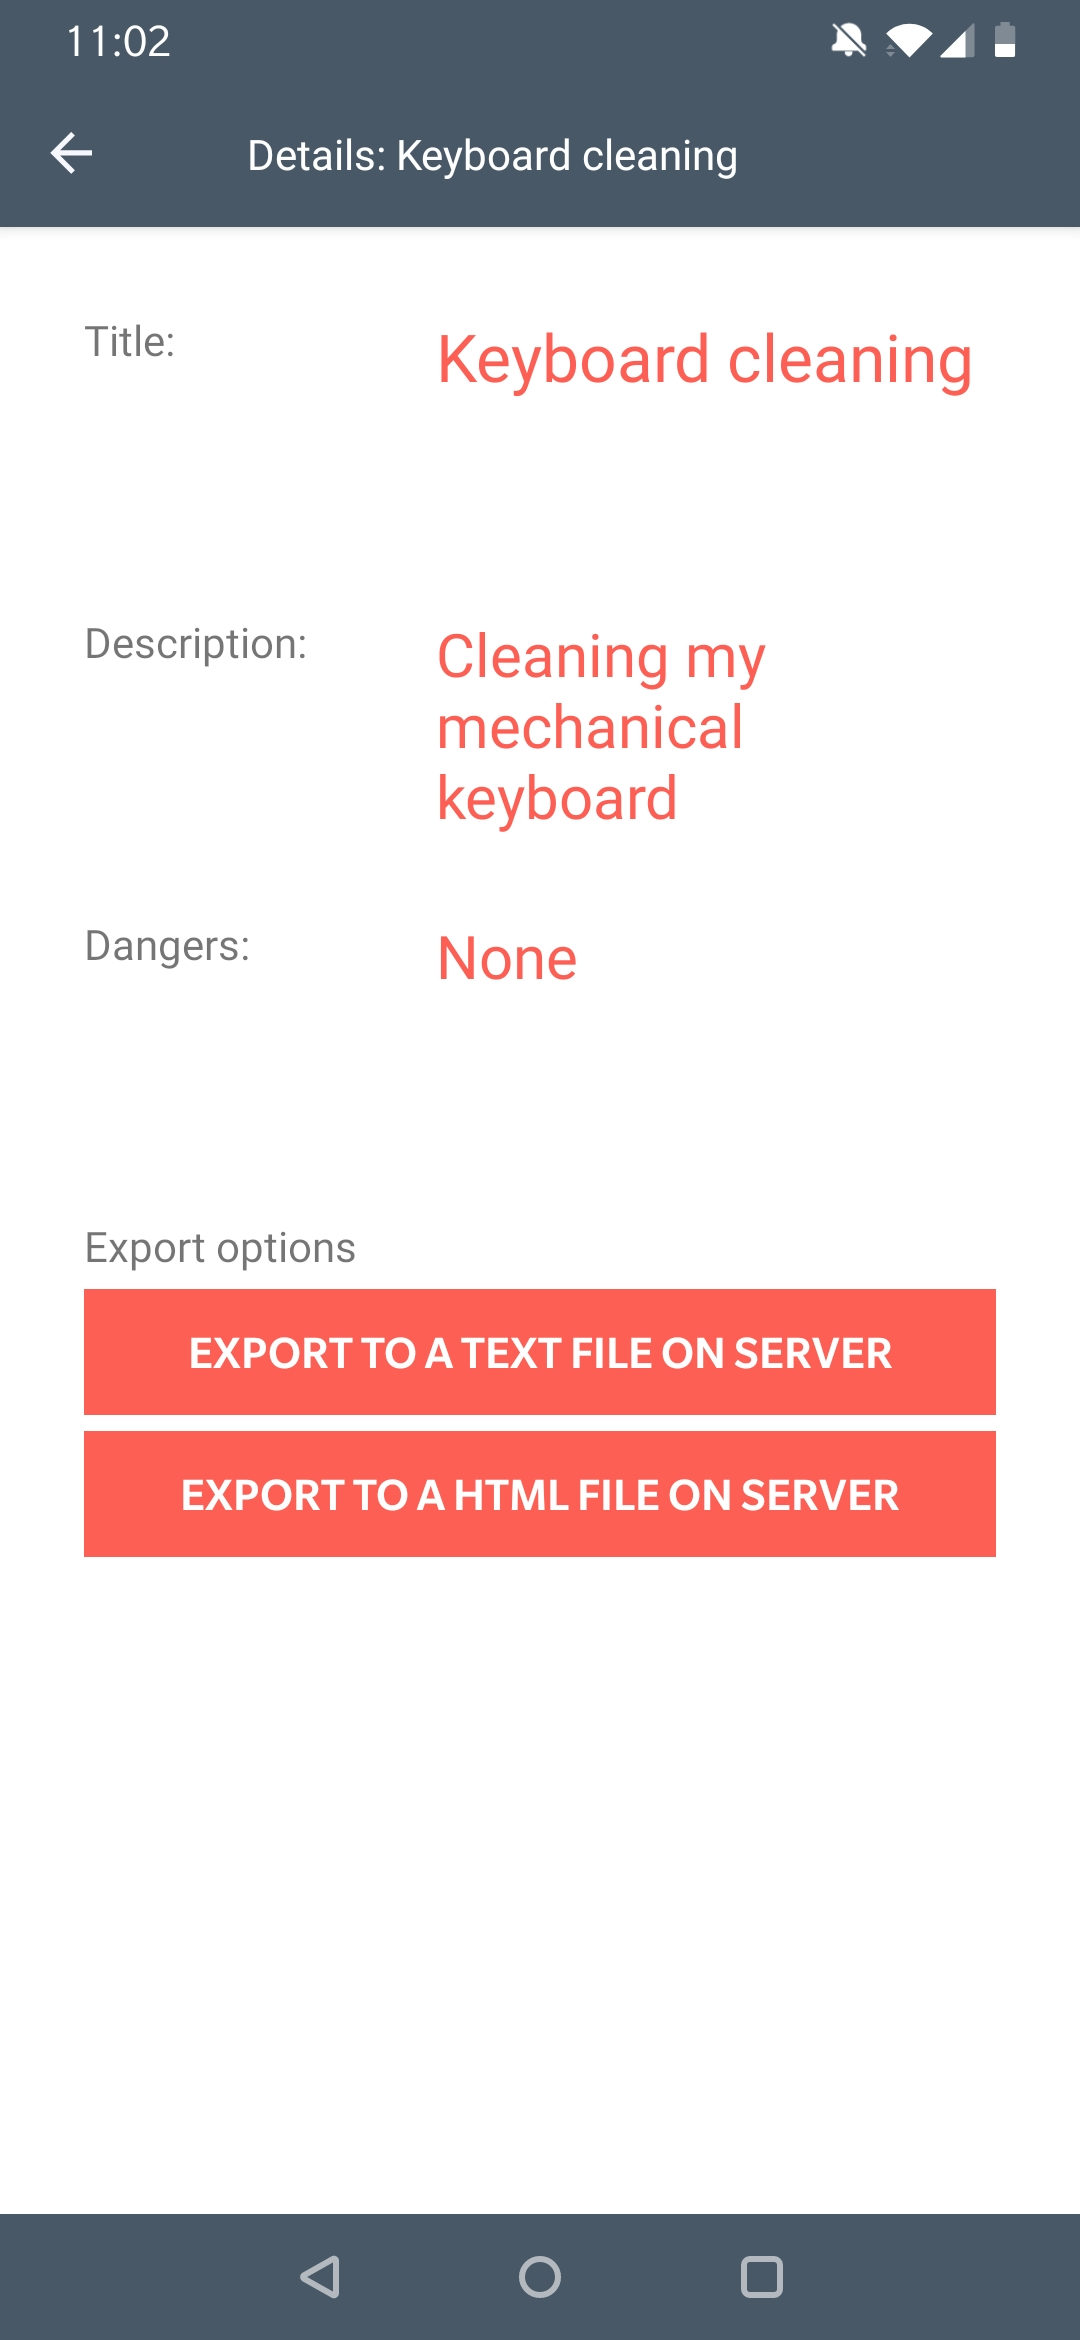
\includegraphics[width=4cm]{app_project_export}
\end{center}
	\caption{Stran za izvoz projektov}
\label{app_note}
\end{figure}

Storitev za komunikacijo s strežnikom pošlje avtoriziran POST zahtevek na strežnik (''\texttt{/project/\{id\}/export/text}'' ali ''\texttt{/project/\{id\}/export/html}'').

\section{Testiranje sistema OpenReport}

\subsection{Testne situacije}

Pripravili smo štiri testne situacije.

\begin{enumerate}
	\item Izdelava opisa tehnološkega postopka \textbf{brez uporabe glasovnega asistenta}
		\begin{enumerate}
			\item brez premora med koraki in
			\item z 90 sekundnim premorom med koraki.
		\end{enumerate}
	\item Izdelava opisa tehnološkega postopka \textbf{z uporabo glasovnega asistenta}
		\begin{enumerate}
			\item brez premora med koraki in
			\item z 90 sekundnim premorom med koraki.
		\end{enumerate}
\end{enumerate}

Z 90 sekundnim premorom smo simulirali delo na izdelku.
Med premorom vpišemo testne podatke v obrazec za dodajanje koraka.
Po 90 sekundnem premoru korak vstavimo v poročilo.

Uporabnik v testni situaciji v poročilo vstavi 4 tekstovne korake in enega slikovnega.
Pri situacijah z uporabo Alexe, mora uporabnik obrazce za korake odpreti z glasovnim ukazom.

\subsection{Metoda testiranja in vpliv na hipotezo}

Testne situacije brez premorov so služile za preverjanje hitrosti dela.
Hipotezo bi potrdili, če bi poročilo napisali prej z uporabo Alexe kot brez nje.

Če bi uporaba Alexe podaljšala čas pisanja, bi hipotezo deloma ovrgli in prešli na drugo stopnjo testiranja.
V drugi stopnji dodamo prejšnjemu postopku 90 sekundni premor med koraki.
Ta premor simulira delo na izdelku.

Če bomo v tej situaciji poročilo z Alexo pisali enako hitro ali hitreje kot brez Alexe, hipoteza ostane delno ovržena.
Če bo pisanje z Alexo počasnejše, kljub dodatnim premorom, pa se bo hipotezo v celoti ovrglo.

\subsubsection{Testni koraki}

\noindent Testni korak za dodajanje tekstovnega koraka je potekal tako:
\begin{enumerate}
	\item premik do mobilnega telefona (3 metre),
	\item odpiranje forme za dodajanje tekstovnega koraka,
	\item vpis besedila ''Test step text'',
	\item nastavitev trajanja na 10 minut,
	\item vstavljanje koraka,
	\item odmik od mobilnega telefona (3 metre).
\end{enumerate}

\noindent Testni korak za dodajanje slikovnega koraka je potekal tako:
\begin{enumerate}
	\item premik do mobilnega telefona (3 metre),
	\item odpiranje forme za dodajanje slikovnega koraka,
	\item zajem slike,
	\item vpis besedila ''Test step text'',
	\item nastavitev trajanja na 10 minut,
	\item vstavljanje koraka,
	\item odmik od mobilnega telefona (3 metre).
\end{enumerate}


\subsection{Rezultati testiranja}

\noindent\begin{tabular}{p{0.2\textwidth}|p{.3\textwidth}|p{.4\textwidth}}    % po potrebi razširi prvo kolono tabele na račun drugih dveh!
  {\bf } & {\bf brez premorov}                             & {\bf z 90 sekundnimi premori} \\ \hline
  {\bf brez Alexe} & 1 minuta 51 sekund & 7 minut 30 sekund \\
  {\bf z Alexo} & 2 minuti 31 sekund & 7 minut 30 sekund \\
\end{tabular}

\bigbreak
\bigbreak
\noindent Iz tega sklepamo, da je hipoteza
\noindent Iz tega sklepamo, da je hipoteza
\noindent Iz tega sklepamo, da je hipoteza
Meritve časa pisanja poročil so pokazale, da je uporaba sistema OpenReport brez Amazon Alexe hitrejša v situaciji brez 90 sekundnih premorov.
To našo hipotezo delno ovrže.
V situacijah z 90 sekundnimi premori, je zapis korakov s pomočjo Amazon Alexe trajal enako dologo kot brez nje.
To našo hipotezo pusti delno ovrženo.
V testnih situacijah Amazon Alexa dela ne pospeši, hkrati pa ga v situaciji s premori ne ovira.

Iz uporabniškega stališča prinese uporaba glasovnega asistenta v proces interakcije z računalnikom novo dimenzijo.
V našem primeru smo lahko zahtevo za odpiranje vnosnega obrazca v mobilni aplikaciji izvedli že na poti do naprave.
V naprednejših izvedbah računalniških sistemov z upravljanjem preko glasovnega asistenta bi lahko olajšali delo slabovidnim in gibalno omejenim posameznikom.



\section{Evalvacija funkcionalnosti}

Primerjali smo pisanje opisa tehnološkega postopka na list papirja, s pisarniškim programom in s sistemom OpenReport z uporabo glasovnega asistenta in sistemom OpenReport brez uporabe glasovnega asistenta.

Mobila aplikacija in strežnik sta izpolnila pričakovanja.
Možnost pisanja tekstovnih korakov služi dobro za manjše opombe.
Slikovni koraki se dobro obnesejo za večje oporne točke pri delu.

Možnost izvoza projekta omogoča tudi prenos podatkov v drugačne sisteme za vodenje evidence dela ali pisanje opisa tehnološkega postopka.

Učinkovitost sistema se z uporabo glasovnega asistenta ni izboljšala.

Pod pričakovnanji se je izkazalo narekovanje besedila glasovnemu asistentu.
Razpoznavanje glasu pri ''Skill-ih'' za asistenta Amazon Alexa deluje najbolje, ko ima stavek veliko stopnjo ujemanja z definirano frazo.
\begin{itemize}
	\item Alexa je frazo ''Take a picture'' pravilno razpoznala v 18 od 20 testnih izgovorjav.
	\item Frazo ''Create a text note'' je pravilno razpoznala v 17 od 20 testnih izgovorjav.
	\item Frazo ''note this is a voice note'' je pravilno razpoznala v 3 od 20 testnih izgovorjav.
	\item Frazo ''note backplate removal takes about three minutes'' ni pravilno razpoznala v nobeni od 20 testnih izgovorjav.
\end{itemize}

Dodajanje slikovnih in teksovnih korakov s pomočjo glasovnega ukaza se je izkazalo za delno uspešno.
Uporabno je bilo predvsem, ko mobilnega telefona med delom nismo imeli na dosegu roke.
Kljub temu je problem prikazovalo dejstvo, da je izgovorjava invokacijske fraze, fraz namer in čakanje na obdelavo zahtev, trajalo v povprečju 18 sekund.


Odklepanje mobilnega telefona, ki ga imamo v dosegu rok in ga lahko dosežemo brez presedanja ter odpiranje forme za dodajanje korakov je trajalo v povprečju 4 sekunde.
Odklepanje mobilnega telefona, ki je oddaljen dva metra ter odpiranje forme za dodajanje korakov je trajalo povprečju 8 sekund.

\chapter{Možnosti nadaljnega razvoja}

Glavna šibka točka sistema OpenReport je bil glasovni asistent Amazon Alexa.

Veliko večjo učinkovitost bi lahko dosegli s specializiranim asistentom, ki bi lahko razpoznal ukaze z eno samo frazo in ne kombinacijo dveh, kot Amazon Alexa.

Boljšo uporabniško izkušnjo bi dosegli tudi s krajšimi prekinitvami za procesiranje ukaza.
Ker Amazon Alexa procesira ukaz na oddaljenem strežniku, so večsekundne prekinitve prikazovale precejšnjo oviro.


%  Veliko bolje bi bilo tudi uporabiti algoritme za razpoznavanje govora brez opore definiranih fraz.

\chapter{Zaključek}


\newpage %dodaj po potrebi, da bo številka strani za Literaturo v Kazalu pravilna!
\ \\
\clearpage
\addcontentsline{toc}{chapter}{Literatura}

\printbibliography

\end{document}
